%%%%%%%%%%%%%%%%%%%%%%%%%%%%%%%%%%%%%%%%%%%%%%%%%%%%%%%%%%%%%%%%%%%%
%% I, the copyright holder of this work, release this work into the
%% public domain. This applies worldwide. In some countries this may
%% not be legally possible; if so: I grant anyone the right to use
%% this work for any purpose, without any conditions, unless such
%% conditions are required by law.
%%%%%%%%%%%%%%%%%%%%%%%%%%%%%%%%%%%%%%%%%%%%%%%%%%%%%%%%%%%%%%%%%%%%

\documentclass[
digital, %% This option enables the default options for the
%% digital version of a document. Replace with `printed`
%% to enable the default options for the printed version
%% of a document.
table,   %% Causes the coloring of tables. Replace with `notable`
%% to restore plain tables.
lof,     %% Prints the List of Figures. Replace with `nolof` to
%% hide the List of Figures.
lot,     %% Prints the List of Tables. Replace with `nolot` to
%% hide the List of Tables.
%% More options are listed in the user guide at
%% <http://mirrors.ctan.org/macros/latex/contrib/fithesis/guide/mu/sci.pdf>.
oneside,
]{fithesis3}
%% The following section sets up the locales used in the thesis.
\usepackage[resetfonts]{cmap} %% We need to load the T2A font encoding
\usepackage[T1,T2A]{fontenc}  %% to use the Cyrillic fonts with Russian texts.
\usepackage[
main=czech,  %% By using `czech` or `english` as the main locale
%% instead of `slovak`, you can typeset the thesis
%% in either Czech or English, respectively.
english, german, russian, czech, slovak %% The additional keys allow
]{babel}        %% foreign texts to be typeset as follows:
%%
%%   \begin{otherlanguage}{german}  ... \end{otherlanguage}
%%   \begin{otherlanguage}{russian} ... \end{otherlanguage}
%%   \begin{otherlanguage}{czech}   ... \end{otherlanguage}
%%   \begin{otherlanguage}{slovak}  ... \end{otherlanguage}
%%
%% For non-Latin scripts, it may be necessary to load additional
%% fonts:
\usepackage{paratype}
\def\textrussian#1{{\usefont{T2A}{PTSerif-TLF}{m}{rm}#1}}
%%
%% The following section sets up the metadata of the thesis.
\thesissetup{
date            = \the\year/\the\month/\the\day,
university      = mu,
faculty         = sci,
department      = Ústav chemie,
departmentEn    = Department of Chemistry,
extra = {
departmentCs  = Department of Chemistry,
},
programme       = Fyzikální chemie,
programmeEn     = Physical Chemistry,
extra = {
programmeCs   = Chemistry,
},
field           = Fyzikální chemie,
fieldEn         = Physical Chemistry,
extra = {
fieldCs       = Physical Chemistry,
},
type            = mgr,
author          = Petra Hrozková,
gender          = f,
advisor         = doc. Markéta Munzarová Dr. rer. nat. ,
title           = Studium elektronové struktury fosfosilikátů a~jejich silikátových          prekurzorů metodou DFT,
TeXtitle        = Studium elektronové struktury fosfosilikátů a~jejich silikátových          prekurzorů metodou DFT
.
,
titleEn         = A~DFT study of the Electronic Structure of Silicate Precursors for Phosphosilicates
,
TeXtitleEn      = A~DFT study of the Electronic Structure of Silicate Precursors for Phosphosilicates
,
extra = {
titleCs       = Studium elektronové struktury fosfosilikátů a~jejich silikátových prekurzorů metodou DFT
,
TeXtitleCs    = Studium elektronové struktury fosfosilikátů a~jejich silikátových prekurzorů metodou DFT
,
},
keywords        = {silikofosfáty, hypervalence, DFT, HSAB, NBO, MPA, nmr posun},
TeXkeywords     = {silikofosfáty, hypervalence, DFT, HSAB, NBO, MPA,  nmr posun \ldots},
keywordsEn      = {silicophospahtes, hypervalency,DFT, HSAB, NBO, MPA, nmr shifts ...},
TeXkeywordsEn   = {silicophospahtes, hypervalency,DFT, HSAB, NBO, MPA,  nmr shifts, \ldots},
extra = {
keywordsCs    = {silikofosfáty, hypervalence, DFT, HSAB, NBO, MPA, nmr posun},
TeXkeywordsCs = {silikofosfáty, hypervalence, DFT, HSAB, NBO, MPA, nmr posun},
},
abstract      = {Práce je zaměřená na studium silikofosfátů a~reaktantů používaných v~jejich přípravě. Studované struktury jsou rozděleny podle velikosti na tři části. Malé modely reprezentují blízké okolí křemíku v~silikofosfátech a~zároveň jsou sem zahrnuty i reaktanty, které byly používány v~experimentálních pracích. Střední modely již obsahují cykly a~velké modely reprezentují výsek ze skutečných silikofosfátových polymerů. Strukutury jsou studovány na úrovni teorie funkcionálu hustoty. První cíl je porovnat sklon k~hypervalenci na základě teorie HSAB a~to podle hodnot globální tvrdosti $\eta$ a~absolutní elektronegativity $\chi$. Je zde púozorována korelace mezi $\chi$ a~ochotou sloučenin navyšovat koordinaci.

Další část práce je určich ochotu tvořit hypervalentní sloučeniny na základě složení vazebných a~protivazebných orbitalů. Pomocí Mullikeonovy populační analýzy jsou analyzovány vazebné orbitaly a~podle teorie přirozených orbitalů je určeno složení protivazebných orbitalů. Pro sloučeniny s~nižší hodnotou $\chi$ je pozorováno menší zapojení křemíku do protivazebných orbitalů, které jsou klíčové pro Lewisovskou kyselost.

Poslední část práce se věnuje modelům, které popisují již rozsáhlejší silikofosfátovou síť. Modely zde vychází z~dat z~rentgenové krystalografie a~experimentálních chemických posunů. Zároveň je zde snaha modelovat zapojení acetátových skupin do struktur silikofosfátů a~modelováné pětikoordinovaných strukutr křemíku. Správnost modelů je ověřena na základě shody rozdílu v~chemických posunech pro jednotlivé koordinace. Větší síťování struktur odpovídá zápornějším hodnotám chemikých posunů.

},
abstractEn    = {This is the English abstract of my thesis, which can

span multiple paragraphs.},
extra = {
abstractCs   = {This is the Czech abstract of my thesis, which can

span multiple paragraphs.},
},
thanks        = {Tato práce vznikla za podpory projektů CERIT Scientific Cloud (LM2015085) a~CESNET (LM2015042) financovaných z~programu MŠMT Projekty velkých infrastruktur pro VaVaI.},
bib           = example.bib,
%% Uncomment the following line (by removing the % symbol at
%% the beginning) and replace `assignment.pdf` with the
%% filename of your scanned thesis assignment.
% assignment    = assignment.pdf,
}
\usepackage{makeidx}      %% The `makeidx` package contains
\makeindex                %% helper commands for index typesetting.
%% These additional packages are used within the document:
\usepackage{paralist} %% Compact list environments
\usepackage{amsmath}  %% Mathematics
\usepackage{amsthm}
\usepackage{amsfonts}
\usepackage{url}      %% Hyperlinks
\usepackage{mhchem}
\usepackage{chemfig}
\usepackage{subfigure}
\usepackage{listings} %% Source code highlighting
\usepackage{braket}
\usepackage{tikz}
\usepackage{verbatim}
\usepackage{footmisc}

\renewcommand{\thesubfigure}{}
%\usepackage{subcaption}
\usepackage{graphicx}
\usetikzlibrary{patterns}
\DeclareRobustCommand{\legendsquare}[1]{%
\tikz[baseline=(a.south)]{\node[#1, inner sep=.8ex, outer sep=0] (a) {};}%
}
\usepackage{etoolbox}

\newrobustcmd*{\mycircle}[1]{\tikz{\filldraw[draw=#1,fill=#1] (0,0) circle [radius=0.1cm];}}
\newrobustcmd*{\mycircleempty}[1]{\tikz{\draw (0,0) circle [radius=0.1cm];}}
\DeclareUnicodeCharacter{2009}{ }% support older LaTeX versions
\DeclareUnicodeCharacter{2212}{ }% support older LaTeX versions
\DeclareUnicodeCharacter{2192}{$\rightarrow$}
\DeclareUnicodeCharacter{2190}{$\leftarrow$}
\DeclareUnicodeCharacter{2032}{`}


%\renewcommand{\baselinestretch}{1.2}
%\usepackage{chemmacros}

\lstset{
basicstyle      = \ttfamily,%
identifierstyle = \color{black},%
keywordstyle    = \color{blue},%
keywordstyle    = {[2]\color{cyan}},%
keywordstyle    = {[3]\color{olive}},%
stringstyle     = \color{teal},%
commentstyle    = \itshape\color{magenta}}
\usepackage{floatrow} %% Putting captions above tables
\floatsetup[table]{capposition=top}

\begin{document}
\chapter*{Seznam zkratek}
\begin{table}[htbp]
%\begin{center}
\begin{tabular}{l l}
  BD & Bond Orbitals \\
CC & Coupled Cluster \\
CI & Configuration Interaction \\
DFT & Density Funkcional Theory \\
ECP & Effective Core Potentials \\
GGA &  Generalized Gradient Approximation \\
GTO & Gaussian Type Orbitals \\
HF-SCF & Hartree-Fock Self-Consistend Field \\
HOMO  & Highest Occupied Molecular Orbital \\
HSAB & Hard and Soft Acids and Bases \\
IGLO & Individual Gauge for Localized Orbitals \\
LDA & Local-density approximation \\
LSDA & Local Spin Denstiy Approximation \\
LUMO & Lowest Unoccupied Molecular Orbital \\
MPA & Mulliken Population Analysis \\
MBPT &  Many-Body Perturbation Theory \\
MO-LCAO & Molecular Orbital – Linear Combination of Atomic Orbitals \\
NBO & Natural Bond Orbitals \\
QM & Quantum Mechanics \\
SD & Slaterův Determinant \\
STO & Slater-type orbital  \\
\end{tabular}
%\end{center}
\end{table}

\chapter{Experimentální motivace}
%\section{}
Cílem této práce je podat vysvětlení některých experimentálních jevů, které byly pozorovány u~silikofosfátových polymerů. Studium vysoce porézních silikofosfátů je jedním ze zaměření skupiny anorganické a~materiálové chemie na našem ústavu. Studie prezentované v~této práci se zaměřují na na přítomnost hypervalentního, tj. pěti nebo šestikoordinovaného křemíku, v~jednotlivých strukturách. Obecný pohled na hypervalency poskytuje Rundleovo a~Piementelovo schéma, kde se objevují elektronově-bohaté tří-centerní vazby \cite{405827} \cite{Munzarova2001}.

Amorfní struktura silikofosfátových xerogelů však neumožňuje jejich přímou strukturní charakterizaci. Důležitou součástí práce bylo navržení vhodných strukturních modelů. Modely navržené v~této práci byly motivovány rentgenovými strukturami analogických periodických struktur z~prací \cite{C3NJ00721A}, \cite{rtg_4_pinkas} anebo příbuznými strukturami, které budou dále popsány. Dále byla využita data z~NMR spektroskopie, z~nichž byly odvozeny informace o~výši koordinace křemíku a~složení ligandů (fosfátové vs. organické estery)\cite{Styskalik2015thesis}. Druhou součástí práce byl podrobnější pohled na chemickou vazbu ve zvolených modelech silikofosfátových polymerů. Pro analýzu chemické vazby byla použita teorie přirozených orbitalů a~Mullikenova populační analýza.

\section{Silikofosfátové polymery}
Nejčastější formou výskytu křemíku v~přírodě jsou křemičitany, sloučeniny obsahující křemík tetraedricky koordinovaný čtyřmi atomy kyslíku. Existují však i minerály s~vyšší koordinací, např. thaumasit \cite{Edge:a08100}. Vzhledem k~vysokému významu křemíku v~přírodě jsou křemičitany rozsáhle připravovány a~studovány i laboratorně. Oxid křemičitý \ce{SiO2} je po vodě nejvíce studovanou sloučeninou. Díky tomu, že \ce{Si^4+} je velikostně snadno zaměnitelný za \ce{Al^3+} nebo \ce{P^5+}, vznikají pak hlinitokřemičitany, obsahující Si-O-Al (zeolity), nebo fosfokřemičitany, obsahující Si-O-P, tj. silikofosfáty. Obě skupiny sloučenin jsou rozsáhle studovány. Konkrétně silikofosfátové polymery mají zajímavé fyzikální a~chemické vlastnosti. Příkladem je Brønstedovská kyselost nebo vysoká protonová vodivost. Několik z~možných uplatnění silikofosfátových polymerů mohou být konduktory, elektrolyty, optická vlákna a~biokompatibilní materiály.\\

Silikofosfáty i hlinitokřemičitany jsou charakteristické svojí trojrozměrnou  porézní strukturou. Naše pozornost je v~této práci soustředěna na silikofosfáty. Předpokládaná struktura připravených silikofosfátů studovaných v~předchozích experimentálních pracích Aleše Stýskalíka je znázorněna na obrázku \ref{si_polymer_cely} \cite{Styskalik2015thesis}. Charakteristickou vlastností struktur silikofosfátů je uspořádání jednotek Si-O-P do cyklů, struktury s~hypervalentním křemíkem obsahující osmičlenné cykly vzniklé dvojnásobným opakováním jednotky Si-O-P-O. Již byla ale i experimentálně přípravena struktura s~dvanáctičlennými cykly \cite{velky_cyklus}. Struktura je uvedena na obrázku \ref{velky_cyklus}.

\begin{figure}
\caption{Struktura s~12-členným kruhem nakreslená autorkou DP v~programu Avogadro na základě dat uvedených v~práci \cite{velky_cyklus}.  Struktura byla upravena tak, aby byla viditelná existence 12-členného cyklu, neboť v~původní prácei chybí konektivita jednoho z~atomů fosforu do cyklu.;  Legenda: \mycircle{brown} Si, \mycircle{red}~O, \mycircle{orange}~C, \mycircle{yellow} P, \mycircleempty{black}~H.}
\center \includegraphics[width=9cm]{si_velky_kruh.png} \label{velky_cyklus} \end{figure}

\begin{figure}
\caption{Struktura \ce{[(Ph2Si{O2P(O)OSiMe3})2]} získaná pomocí rentgenové krystalografie v~práci \cite{rtg_4_pinkas};  Legenda: \mycircle{brown} Si, \mycircle{red}~O, \mycircle{orange}~C, \mycircle{yellow} P, \mycircleempty{black}~H, \mycircleempty{blue}~N .}
\center 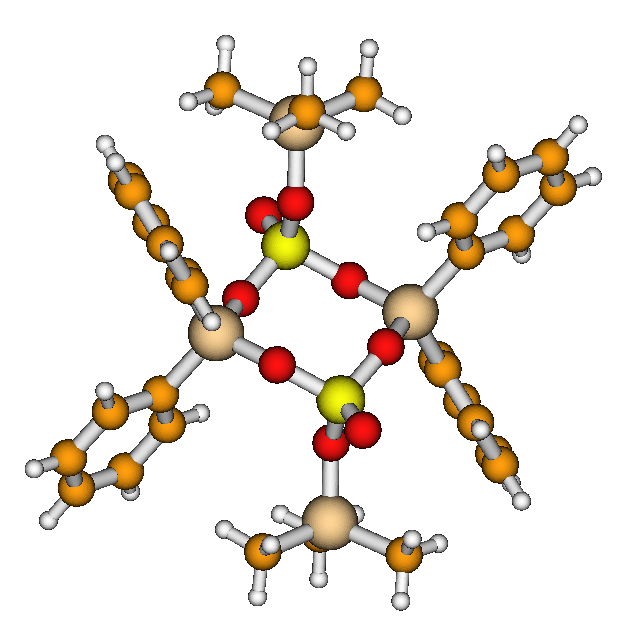
\includegraphics[width=6cm]{rtg_kruh_samostatne.png} \label{rtg_cyklus} \end{figure}
Obrázek \ref{si_polymer_cely} znázorňuje předpokládanou strukturu silikofosfátového xerogelu se třemi druhy křemíkových center (koordinace čtyřmi fosfáty, šesti fosfáty, anebo čtyřmi fosfáty a~dvěma organickými estery současně) a~osmičlennými cykly Si-O-P.  Konkrétní podoba osmičlenného cyklu byla ověřena metodou RTG viz. obrázek \ref{rtg_cyklus}, \cite{rtg_4_pinkas}. Stupeň koordinace křemíku a~současně velikost pórů se ukázala být silně závislá na typu prekurzoru. Pokud byl ve výchozích sloučeninách jeden z~fosfátů nahrazen methylovou skupinou přímo vázanou na křemík, ve výsledném xerogelu se nevyskytovaly oktaedricky koordinované křemíky a~velikost pórů byla větší. Konkrétní podobu okolí křemíku je ukázáno ve schématu na obrázku \ref{si_polymer_cely}. Podoba koordinačního okolí byla získána pomocí NMR dat z~prací \cite{rtg_4_pinkas} a~\cite{Styskalik2015thesis}. Silikofosfátové cykly jsou pak dále organizovány do vyšších struktur mikroporézního (šířka pórů do 2 nm) až mezoporézního (šířka póru 2-50~nm) skeletu. Potvrzená struktura šestikoordinovaného křemíku je uvedena na obrázku \ref{rtg_koordinace_sest} \cite{C3NJ00721A}. Struktura byla získána metodou rentgenové difrakce. Konkrétní metody příprav slikofosfátových sloučenin jsou uvedeny například v~práci Aleše Stýskalíka \cite{Styskalik2015thesis}.

\begin{figure}
\caption{Silikofosfátová síť v~práci \cite{Styskalik2015thesis}.}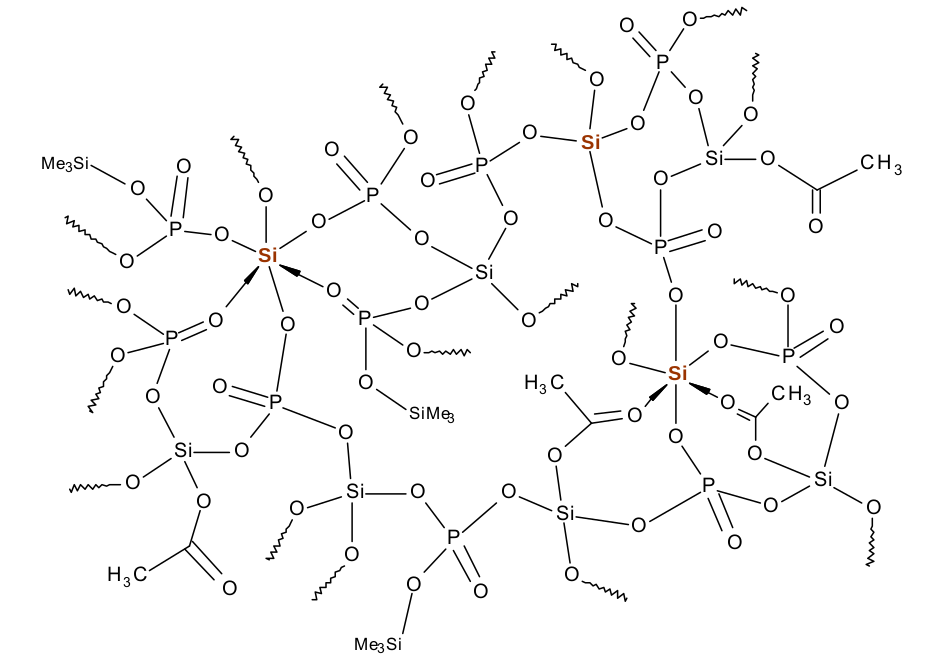
\includegraphics[width=10cm]{si_polymer_cely.png}
\label{si_polymer_cely}\end{figure}
\begin{figure}
\caption{Struktura\ce{(Si^{VI}(PO4)6(Si^{IV}O4Et2)6)^{2-}} získaná rentgenovou krystalografií v~práci \cite{C3NJ00721A};  Legenda: \mycircle{brown} Si, \mycircle{red}~O, \mycircle{orange}~C, \mycircle{yellow} P, \mycircleempty{black}~H. }
\center \includegraphics[width=8cm]{obr_si_kryst_struktura_real.png} \label{rtg_koordinace_sest} \end{figure}

\section{Hypervalence $p$-prvků}
První kvantitativní popis chemické vazby zavedl Lewis v~roce 1916, kdy vazbu považoval za sdílení elektronového páru mezi dvěma atomy. Cílem párování bylo zaplnění valenčí vrsty a~dosažení konfigurace vzácného plynu, tvz. oktetové pravidlo. Pravidlo elektronového oktetu říká, že  prvky $p$ skupiny chtějí mít ve své valenční vrstvě právě osm elektronů. Toho lze docílit vytvořením chemické vazby, excitací nebo ionizací. Spárované elektrony, které se neúčastní vazby, se nazývají volné elektronové páry. Přísná lokalizace elektronů s~pomocí vazebných orbitalů v~Lewisovské teorii ovšem nesouhlasila s~pozorováním pro organické sloučeniny s~uhlíkem. Vysvětlení podal L. Pauling pomocí teorie valenčních vazeb a~teorie hybridizace \cite{Munzarova1996thesis}.\\

Podle klasické teorie valenční vazby mohou $p$ prvky tvořit čtyři vazby. Z~experimentálního pozorování je ale známo, že prvky $p$ bloku tvoří i více vazeb než je číslo jejich atomových orbitalů, obvykle pět nebo šest. Příkladem můhou být sloučeniny xenonu, například \ce{XeF6}.
Sloučeniny, kde se vyskytuje jeden nebo více atomů s~více než osmi elektrony (oktet) se nazývají hypervalentní/hyperkoordinované. Konkrétně křemík může vytvářet čtyř, pěti a~šestikoordinované sloučeniny a~stát se hypervalentní. Pro vysvětlení hypervalence $p$ prvků lze použít teorii hybridizace. Obecně se čtykoordinované sloučeniny vyskytují jako tetraedry, hybridizace $sp^3$. Pětikoordinované sloučeniny tvoří trigonální bipyramidu, hybridizace $sp^3d$. A~šestikoordinované sloučeniny tvoří oktaedr, hybridizace $sp^3d^2$. Přehled navyšování koordinace křemíku je uveden na obrázku \ref{prehled_koordinaci}.

\begin{figure}
\caption{Přehled navyšování koordinací křemíku.}
\center 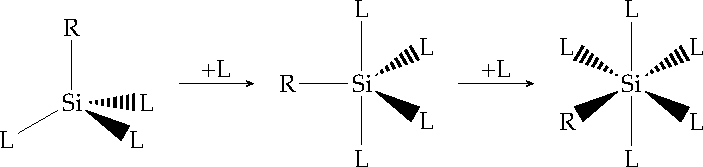
\includegraphics[width=10cm]{drawing.pdf} \label{prehled_koordinaci} \end{figure}

Čtyřkoordinovaný křemík splňuje tetraedrické uspořádání. Při zvýšení koordinace na pět by měla být pozorována trigonální bipyramida, $sp^3d$. Výskyt $d$ orbitalů ve vazbě ale způsobuje nárust energie vazby na více než 200 kcal/mol. Z~tohoto důvodu se předpokládá, že $d$ orbitaly se podílejí pouze na polarizaci $p$ orbitalů. Pentavalentní koordinace by měla být realizována jako $3sp^2$ hybridizace doplněna třícenterní, čtyřelektronovou vazbou $3c-4e$ s~$p$ orbitalem. V~pětikoordinovaných sloučeninách se ale spíše uvažuje hybridizace $sp^2$ a~jedna vazba $3c-4e$ s~$p$ orbitalem, právě kvůli energii $d$ orbitalů.

Hypervalentní sloučeniny jsou lepší Lewisovské kyseliny díky $d+$ efektu na centralním křemíku. Důvodem je přesun elektronové hustoty na ligandy skrz nevazebné MO a~podpora $3c-4e$ vazby. Rozložení elektronové hustoty molekulu stabilizuje a~z~tohoto důvodu se v~hypervalentních sloučeninách vyskytují jako ligandy prvky s~vysokou elektronegativitou. Tento jev dobře popisuje tzv. Bentovo pravidlo:"Elektronegativní prvek dáva přednost vazbě s~větším p-charakterem" \cite{hypervalentsiliconmacmillangroup2005}. Pro křemík v~koordinaci šest lze také předpokládat, že význam $d$ orbitalů nebude významný vzhledem k~jejich energii. I~zde se do vazby zapojí $3c-4e$ vazby \cite{Wagler2014}.

Další možnost interpretace hypervalence je založena na vysoké iontovosti vazby na křemíku. Obecně iontovost s~koordinačním číslem roste.
Navíc chování vazby Si-ligand silně závisí na samotném ligandu a~sterickém a~elektronovém uspořádání. Hovoříme o~Lewisovské kyselosti křemíkové vazby s~elektronegativním atomem. Chování křemíku lze rozdělit na iontové, sigma vazebné a~donor s~interakcí \cite{Wagler2014}.\\

\section{Hypervalence sloučenin křemíku}\label{teorie_hypervalence}
V~případě čtyřkoordinovaných sloučenin poskytuje křemík do vazeb všechny své valenční elektorny. Ve vyšším koordinačním stupni už může křemík poskytnou pouze prázdné orbitaly a~proto se chová jako Lewisovská kyselina. Obecně mají Lewisovské kyseliny prázdné molekulové orbitaly, které leží dostatečně blízko obsazeným molekulovým orbitalů (MO)\footnote{MO - \textit{Molecular orbital}.} konjugované báze.
\begin{figure}
\begin{center}
\subfigure[]{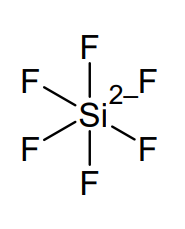
\includegraphics[width=2cm]{si_f6.png}\label{si_f6}}
\subfigure[]{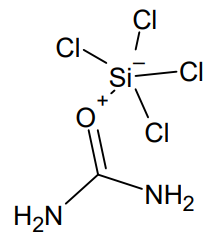
\includegraphics[width=3cm]{si_cl_o.png}\label{si_cl_o}}
\subfigure[]{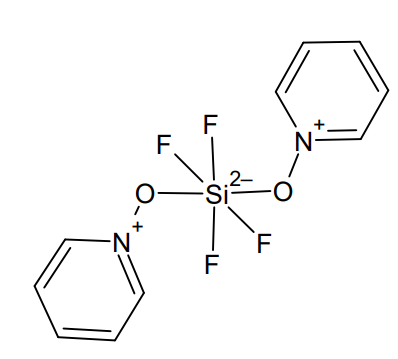
\includegraphics[width=5cm]{si_o_f.png}\label{si_o_f}}
\subfigure[]{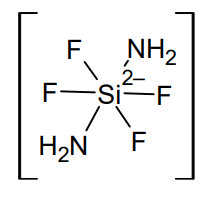
\includegraphics[width=3cm]{si_f_n.png}\label{si_f_n}}
\subfigure[]{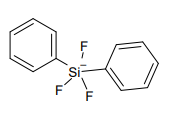
\includegraphics[width=5cm]{si_with_fluor_carbons.png} \label{si_with_fluor_carbons}}
\subfigure[]{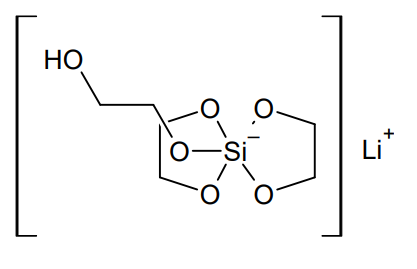
\includegraphics[width=5cm]{si_only_o.png} \label{si_only_o}}
\subfigure[]{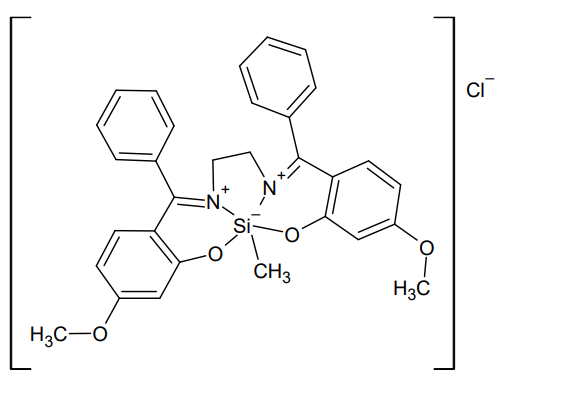
\includegraphics[width=5cm]{si_n_o_c.png}\label{si_n_o_c}}
\subfigure[]{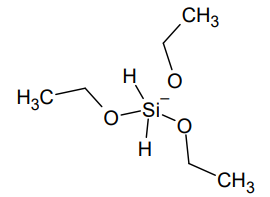
\includegraphics[width=5cm]{si_fluor_vodik_kyslik.png} \label{si_fluor_vodik_kyslik}}
\subfigure[]{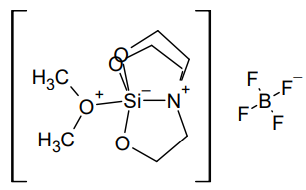
\includegraphics[width=5cm]{si_o_n.png} \label{si_o_n}}
\subfigure[]{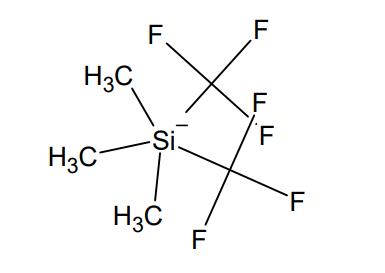
\includegraphics[width=5cm]{si_only_c.png} \label{si_only_c}}
\label{shrnuti_struktury_kremik}
\end{center}
\end{figure}
Z~experimentu je známo, že \ce{SiO4} je dostatečnou Lewisovskou kyselinou, aby křemík mohl přímo reagovat s~Lewivoskou bazí. Pokud je jeden z~kyslíku ve struktuře nahrazen uhlíkem, schopnost navyšovat koordinaci je ztracena. Stejný jev pozoroval Aleš Sýskalík a~spol. \cite{Styskalik2015thesis} a~to vedlo k~hypotézi o~snížení Lewisovské kyselosti křemíku při tvorbě přímé vazby Si-C. Naopak pětikoordinovaný křemík je lepší Lewisovskou kyselinou než čtyřkoordinovaný křemík a~hypervalency podporuje. Atomy jako uhlík, dusík, kyslík, fluor nebo chlor podporují navyšování koordinace křemíku \cite{Wagler2014}.\\

Existující, experimentálně připravené hypervalentní sloučeniny s~křemíkem lze rozdělit podle jednotlivých ligandů a~jejich poloze v~periodické tabulce. Křemík je schopen tvořit hypervalentní sloučeniny s~fluorem, příkladem může být struktura  \ce{(SiF6)^{2-}} viz. obrázek \ref{si_f6} \cite{memoriesphysiquelussac}. Tato struktura byla připravena v~19. století a~považuje se za první připravenou sloučeninu křemíku v~koordinaci šest. Pokud budeme postupovat ve skupine halogenů dolů, dalším ligandem by měl být logicky chlor. Sloučenina \ce{SiCl6^{2-}} ale není známá, naopak \ce{GeCl6^{2-}} ano. Schopnost atomu tvořit hypervalentní sloučeniny roste ve skupině dolů. Germanium má tedy vysokou schopnost tvořit hypervalentní sloučeniny. Oproti tomu křemík potřebuje ligand s~výrazně vyšší elektronegativitou. Hypervalentní sloučeniny s~chlorem byly proto připraveny až později, viz. obrázek \ref{si_cl_o} \cite{LAZAREV199716}.

Ve sloučeninách s~křemíkem může být fluor nahrazen dalšími $p$ prvky, například kyslíkem viz. obrázek \ref{si_o_f} \cite{C0DT01115K} nebo kyslíkem a~vodíkem viz. obrázek  \ref{si_fluor_vodik_kyslik} \cite{BOYER19812165}.
Jako ligand společně s~fluorem může být použit i dusík viz. obrázek \ref{si_f_n} \cite{C0DT01115K} nebo uhlík viz. obrázek \ref{si_with_fluor_carbons} \cite{kremikfluorcarbon}. Schopnost křemíku navyšovat koordinaci existuje i ve sloučeninách s~kyslíkem viz. obráázek \ref{si_only_o} \cite{flyn1969}.  Struktura \ce{SiO6} se vyskytuje také v~přírodě v~minerálu thaumasitu \cite{Edge:a08100}. Kyslík může být nahrazen dusíkem  viz. obrázek \ref{si_o_n} \cite{Wagler2014} nebo uhlíkem a~dusíkem viz. obrázek \ref{si_n_o_c} \cite{Wagler2014}. Je zajímavostí, že existují i sloučeniny pouze s~vazbou křemík-uhlík viz. obrázek \ref{si_only_c} \cite{A901953G} \cite{Wagler2014}.

\section{Formulace teoretického problému}
Postupně jsme hlavní otázku, řešenou v~této práci, zformulovali do následující podoby: Jaká je souvislost mezi kombinací ligandů na čtyřkoordinovaném křemíku a~Lewisovskou kyselostí těchto čtyřkoordinovaných sloučenin, vedoucí ke sklonu křemíku zvýšit svoji koordinaci na pět nebo šest ligandů.
Z~tohoto důvod jsme se rozhodli porovnávat Lewisovskou kyselost, abychom určili stabilitu jednotlivých částí silikofosfátů. Navíc jsme se snažili najít parametr, který by umožnil určit velikost póru v~závislosti na okolí křemíku. Pro tuto práci jsem zvolila tři úrovně zkoumání silikofosfátů, rozdělené podle velikosti modelů. Velké modely sloužily jako odhad skutečné struktury silikofosfátů, včetně jednotlivých pórů. Středně velké modely byly stále dost komplexní, ale již umožňovaly podrobnější pohled na chemickou vazbu Si-C. Malé modely byly snadné pro porozumění.

Jako prostředek ke zkoumání silikofosfátů jsem zvolila molekulové orbitaly, které poskytují široké spektrum informací o~molekule, vazbách, struktuře, kyselosti, \dots.  Analýza byla provedena s~pomocí teorie funkcionální hustoty (DFT)\footnote{DFT - \textit{Density Functional Theory}, česky Teorie funkcionálu hustoty.}, která se řadí mezi kvantově-chemické metody. Pro porovnání byla stejná analýza udělána s~pomocí teorie přirozených molekulových orbitalů (NBO)\footnote{NBO - \textit{Natural Bond Orbitals.}, česky Přirozené Molekulové orbitaly}. Výhoda přístupu NBO je snadnější převod číselných výsledků do tradičního chemického významu. Pro určení Lewisovské kyselosti bylo stěžejní určení procenta $s$ a~$p$ orbitalů křemíku v~protivazebných orbitalech.  V~NBO analýze jsme určovali procento vazebných orbitalů (BD) \footnote{BD - \textit{Bond Orbital}.} a~protivazebných (BD*) orbitalů křemíku a~ligandu. V~MPA\footnote{MPA - \textit{Mulliken's Population Analysis.}, česky Mullikenova populační analýza} analýze jsme určovali procento $s$~a~$p$ orbitalů křemíku a~okolních ligandech.
\newpage

\chapter{Metody kvantové chemie}
Chování elektronů v~molekulách však nelze popsat rovnicemi ani jazykem klasické mechaniky. Elektrony totiž vykazují typické kvantově-mechanické chování, projevující se diskrétním spektrem energií, vlnovým chováním ve smyslu difrakce nebo např. fotoelektrickým jevem. Nelze je proto charakterizovat jejich jednotlivými polohami a~hybnostmí, jediný přijatelný popis lze udělat pomocí tzv. vlnové funkce.
\section{Kvantově-mechanický popis elektronové struktury}
Současné chápání struktury, reaktivity a~spektroskopického chování látek je založeno na detailní znalosti rozložení elektronů a~jejich energiích v~atomech a~molekulách. Vlnová funkce se zpravidla označuje řeckým písmene $\Psi$ a~je řešením Schrödingerovy vlnové rovnice \ref{schr_rce}. Levá strana Schrödingerovy rovnice vyjadřuje působení tzv. Hamiltoniánu ($\widehat{H}$) neboli operátoru energie na vlnovou funkci $\Psi$. Pravá strana Schrödingerovy rovnice vyjadřuje fakt, že lze nalézt takové vlnové funkce $\Psi$, které se působením operátoru $\widehat{H}$ pouze vynásobí konstantou $E$, která má význam energie. Řešením Schrödingerovy rovnice jsou tedy jednak možné hodnoty energie elektronů sytemu a~jednak samotná vlnová funkce $\Psi$, která v~sobě dle tzv. Bornovy interpretace obsahuje informaci o~rozložení pravděpodobnosti výskytu elektronů v~prostoru.
\begin{equation}
\widehat{H} \Psi = E \Psi,
\label{schr_rce}
\end{equation}
Analytická řešení Schrödingerovy rovnice jsou dostupná pouze pro velmi malý okruh jednoduchých modelových Hamiltoniánů, jejiž nejdůležitějšími reprezentaty jsou kvantově-chemický oscilátor, částice v~jámě, atom vodíku a~kation \ce{H2^{+}}. Dokonce ani pro atomu helia, který obsahuje pouze o~jeden elektron více než atom vodíku, není dostupné plně analytické řešení Schrödingerovy rovnice.

Z~tohoto důvodu je ve fyzikálních i chemických aplikacích nutno použít zjednodušení. Základní aproximací, kterou je třeba aplikovat pro všechny molekuly (včetně zmiňovaného iontu \ce{H2^{+}}, pro nejž lze vlnovou funkci elektronu vyjádřit analyticky) je tzv. Born-Oppenheimerova aproximace (B-O) \ref{B_O_approximace}.
Její podstatou je oddělení pohybu elektronů od pohybu jader a~lze ji dobře vysvětlit na základě termodynamické analogie vratného děje. Je-li například expanze plynu proti vnějšímu tlaku prováděna vratně, pohybuje se píst ve válci tak pomalu, že plyn je stále v~rovnováze s~okolím. Jeho tlak pak závisí pouze na pozici pístu. Podobně se jádra pohybují vzhledem k~elektronům tak pomalu, že elektrony zaujmou pro každé rozmístění jader okamžitě nejvýhodnější rozložení. Proto můžeme energii elektronů považovat za závislou pouze na polohách jader. V~rámci B-O aproximace lze tedy vlnovou funkci zapsat ve tvaru rovnice \ref{B_O_approximace}.
\begin{equation}
\Psi_{r_i,R_{\alpha}} = \Psi_{electronic}(r_i,R_{\alpha}) \cdot \Psi_{nuclear}(R_{\alpha}),
\label{B_O_approximace}
\end{equation}
$R_{\alpha}$ jsou souřadnice jader, $\Psi_{electronic}(r_i,R_{\alpha})$ je elektornová vlnová funkce, zavisející explicitně na polohách elektronů a~parametricky na polohách jader. $\Psi_N(R_{\alpha})$ je jaderná vlnová funkce závislá pouze na polohách jader. $ \Psi_{nuclear}(r_i, R_{\alpha}) $ je celková vlnová funkce \cite{lechamolecularmodeling}.
Vlnová funkce elektronů je řešením Schrödingerovy rovnice, jež v~operátoru energie zahrnuje pro každý elektron jeho kinetickou energii, přitahování elektronu jádry a~jeho odpuzování se všemi ostatními elektrony. Poslední jmenovaný člen řídí pohyb každého elektronu a~je závislý na pohybu všech ostatních elektronů. V~důsledků toho není elektronová Schrödingerova rovnice analyticky řešitelná.\\

Druhou základní aproximací kvantové chemie je přístup, v~němž se okamžitá repulze jednoho elektronu s~druhým nahrazuje repulzí prvního elektornu v~časově rozmazanou distribuci druhého elektronu. Cílem je pak nalézt takové vlnové funkce obou (a~všech dalších) jednotlivých elektronů, aby pro jeden elektron byla vlnová funkce tzv. orbital-optimální z~hlediska minimalizace celkové energie. Tady například vlnová funkce pro elektron jedna musí být optimální mj. vzhledem k~repulzím s~elektronem dvě a~obráceně, vlnová funkce pro elektro dva musí být optimální mj. vzhledem k~repulzím s~elektronem jedna. Celková vlnová funkce daného počtu elektronů, která se vyjadřuje jako tzv. Slaterův determinat (SD) z~obsazených orbitalů, musí být z~tohoto hlediska konzistentní sama se sebou, a~proto se výše pospaná metoda nazývá Hartee-Fockova metoda selkonzistentního pole (HF-SCF) \footnote{HF-SCF - \textit{Hartree-Fock Method Self-Consistent Field}.}. Vlnovou funkci lze zapsat jako Slaterův determinant, který zaručuje antisymetrii vlnové funkce vůči výměně polohových a~spinových souřadnic \ref{Slateruv_determinant}.
\begin{equation}
\psi =  \frac{1}{\sqrt{N!}}\begin{vmatrix}
\psi_1(1)\alpha(1) & \psi_1(1) \beta (1)  & \dots & \psi_{n/2}(1)\beta(1) \\
\psi_1(2)\alpha(2) & \psi_1(2) \beta (2) & \dots & \psi_{n/2}(2)\beta(2) \\
\vdots             & \vdots                           & \ddots & \vdots \\
\psi_1(n)\alpha(n) & \psi_1(n) \beta (n) & \dots & \psi_{n/2}(n)\beta(n)
\end{vmatrix}
\label{Slateruv_determinant}
\end{equation}
$\psi_i$ jsou prostorové části jednotlivých orbitalů, 1,2,\dots n jsou jednotlivé elektrony $i$, $\alpha(i)$ resp. $\beta(i)$ jsou spinové funkce těchto elektronů a~$\frac{1}{\sqrt{N!}}$ je normovací konstanta.

Výsledná vlnová funkce se hledá následujícím způsobem: Na počátku výpočtu je zvolena určitá sada orbitalů, které jsou postupně jednotlivě optimalizovány v~poli elektronové hustoty zbylých orbitalů. Tím získáme novou sadu orbitalů, která se liší od původní sady orbitalů. Celý postup je opakován až do okmažiku, kdy mezi předchozí a~následující sadou orbitalů rozdíly v~energiích a~elektronové hustotě klesnou pod předem zvolenou, dostatečně nízkou mez. Protože jsou výsledné energie vlastními funkcemi tzv. Fockova operátoru, který patří mezi tzv. Hermitovské operátory, jsou vypočítané orbitaly $\Psi_i$ a~$\Psi_j$ příslušející různým vlastním hodnotám energie $\varepsilon_i $ a~$\varepsilon_j$ orthogonální, tj. platí rovnice \ref{ortogonal}. Navíc lze zajistit, aby byly orthogonální každé dvě vlnové funkce příslušející stejné vlastní hodnotě energie $\varepsilon_i$, a~také, aby každá vlnová funkce $\varphi_i$ tj. \ref{ortonormal} byla normovaná.
\begin{equation}
S_{ij} = \int \psi_i * \psi_j dx dy dz = 0,
\label{ortogonal}
\end{equation}
\begin{equation}
S_{ii} = \int \psi_i * \psi_i dx dy dz = 1,
\label{ortonormal}
\end{equation}
Nejnižší energie se hledá pomocí selfkonzistentní metody (viz. výše). Nevýhoda HF-SCF přístupu je fakt, že neuvažuje korelaci elektronového pohybu, tj. fakt, že vybraný elektron nevnímá ostatní elektrony v~jejich časově zprůměrovaném rozložení, nýbrž že vnímá okamžité polohy ostatních elektronů a~přizpůsobuje jim svoji polohu.\\

Korelační energii lze vyjádřit jako rozdíl mezi přesnou nerelativistickou energii a~HF limitou tzv. Hartree-Fockovou limitou, což je energie Slaterova determinant, vyjádřeného v~limitě nekonenčné báze. Ačkoliv korelační energie představuje méně než 1\% celkové tzv. energie elektronů, nemůže být zanedbána, pokud požadujeme chemickou přesnost tj. $1-2$ kcal/mol.

Korelační energii lze do výpočtu zahrnout tak, že výsledná vlnová funkce obsahuje mimo Slaterův determinant pro základnní stav také příspěvky Slaterových determinantů pro excitované stavy. Hovoříme pak o~Post-Hartree-Fockových metodách. Mísením excitovaných determinantů lze započítat třemi základními způsoby. Předně jde o~tzv. metodu konfigurační interakce (CI)\footnote{CI - \textit{Configuration Interaction}}, v~níž jsou příspěvky excitací optimalizovány pomocí variační metody. Jiným možným způsobem započtení excitovaných determinantů je poruchová teorie zavedená M{\o}llerem a~Plessetem. Poslední (a~v~reálné praxi nejpřesnější) metodou zahrnutí korelace pohybu elektronů prostřednictvím jejich excitaci do protivazebných MO je tzv. metoda spřažených klastrů. Její výhoda oproti CI je její správné škálování s~velikostí systému díky tomu, že jednotlivými excitacemi zahrnuje i jejich superpozice. V~současné době se metody spřažených klastrů považují za standard kvantové chemie.


\section{Teorie funkcionálu hustoty}
Systémy studované v~této práci mají za cíl modelovat trojrozměrnou silikofosfátovou síť. Skládají se tedy ze silikátových a~fosfátových jednotek, z~nichž na každou jednotku připadá cca. 50 elektronů. Je proto velice důležité zvolit metodu, která bude spojovat vysokou přesnost s~vysokou výpočetní efektivností. Současně je našim cílem porozumění sklonu křemíku k~hypervalenci, což indikuje pokud možno fyzikálně průzračný jednoelektronový model. Všechny tyto požadavky splňuje Kohn-Shamova formulace metody funkcionálu hustoty\footnote{Z matematické analýzy je funkcionál operátor zobrazení z~množiny funkcí do množiny obecně komplexních čísel.}\cite{Bickelhauptdftreview}.

Základní myšlenka teorie funkcionálu hustoty pohlíží na systém elektronů a~jader ze zcela jiného úhlu než tradiční \textit{ab inito} metody kvantové chemie, zahrnující metodu HF-SCF a~její nadstavby. Posledně zmíněné metody zahajují popis molekuly od znalosti tzv. externího potenciálu (nejčastěji daného polohami a~náboji jader) a~pokračují přes konstrukci Hamiltoniánu, nalezení energií a~vlnových funkcí až k~výpočtu výsledné elektronové hustoty.

Základní teorémy metody funkcionálu hustoty (1. a~2. Hohensberg-Kohnův teorém) ukazují, že lze postupovat i opačně. Výsledná elektronová hustota zpětně jednoznačně určuje externí potenciál, a~tedy i vlnovou funkci a~všechny z~ní odvozené měřitelné vlastnosti. Protože je elektronová hustota funkcí pouze tří souřadnic v~prostoru (a~nevztahuje se narozdíl od vlnové funkce k~jednotlivým elektronům), lze metody funkcionálu hustoty využít k~výpočtům, které jsou do výpočetní náročnosti srovnatelné s~metodou HF-SCF, ale co do přesnosti popisu metodu HF-SCF dalece převyšují \cite{jensen2007introduction}.\\

Moderní DFT\footnote{DFT - \textit{Density Functional Theory}.} metody se začaly objevovat po roce 1964 jako výsledek Hohensberg-Kohnova teorému. Aplikace v~kvantově-chemických výpočtech se datují od 90. let. První Hohenberg-Kohnův teorém (H-K) mluví o~základním stavu. "Vnější potenciál $V_ext$ je až na konstantu jednoznačným funkcionálem $\varrho(\vec{r})$, protože $V_ext$ určuje $\widehat{H}$, je úplný popis mnohačásticového základního stavu jednoznačným funkconálem $\varrho(\vec{r})$."\cite{PhysRev.136.B864} První H-K teorém můžeme schématicky vyjádřit takto:
\begin{equation}
\varrho_0 \Rightarrow \{N, Z_A, R_A\} \Rightarrow \widehat{H} \Rightarrow \Psi_0 \Rightarrow E_0,
\end{equation}
Všechny vlastnosti základního stavu mnohaelektronového systému jsou tedy jednoznačně určeny elektronovou hustotou. Návodem pro získání elektronové hustoty je druhý teorém. Obsahem druhého H-K teorému je variační princip, který lze v~našem kontextu vyjádřit následovně.
\begin{equation}
E_0 < E [\tilde{\varrho}] = T[\tilde{\varrho}] + E_{Ne}[\tilde{\varrho}] + E_{ee}[\tilde{\varrho}],
\end{equation}
Kde $\tilde{\varrho}(\vec{r})$ je zkušební hustota, splňující vazebné podmínky. Pro výpočetní chemii mají větší význam Kohn-Shamovy (K-S) orbitaly, které byly výsledkem geniální myšlenky o~rozdělení funkcionálu. Základní úlohou v~Kohn-Shamově reprezentaci DFT je, jak nalézt orbitaly popisující stavy elektronů v~neinteragujícím referenčním systému. Jinými slovy, jak definujeme tzv. Shamův potenciál $V_s$ tak, že optimální Slaterův determinat pro neinteragující elektrony v~tomto potenciálu poskytuje stejnou elektronovou hustotu jako reálný systém? Pro řešení tohoto problému je užitečné vyjádřit energii jako funkci hustoty následovně:
\cite{jensen2007introduction}\cite{koch2000chemist}.
\begin{equation}
%E(\varrho(\vec{r})) = T_s[\varrho(\vec{r})] + J[\varrho(\vec{r})] + \int V_{EX}(\vec{r})\varrho(\vec{r})d\vec{r} + E_{XC}[\varrho(\vec{r})],
E(\varrho(\vec{r})) = T_s[\varrho(\vec{r})] + J[\varrho(\vec{r})] + E_{Ne}[\varrho(\vec{r}] + E_{XE}[\varrho(\vec{r})],
\label{dft}
\end{equation}
$T_s[\varrho(\vec{r})]$ je kinetická energie navzájem neinteragujících elektronů, snadno získatelná jako součet přes jednotlivé elektrony, $J[\varrho(\vec{r})]$ je klasická Coulombovská repulze oblaku s~$\varrho$.
$E_{Ne}[\varrho(\vec{r}]$ je energie atrakce elektronů jádry. Jediný poslední člen rovnice \ref{dft} $E_{XE}[\varrho(\vec{r})] $ - tzv. výměnně-korelační funkcionál není v~současnosti znám a~analytický tvar musí býr aproximován \cite{parr1994density}.

\subsection{DFT metody v~praxi}
Největším problémem při aplikaci DFT je nalezení vhodného výměně-korelačního potenciálu. V~principu přesný K-S přístup neříká nic o~tom, jak výměně-korelační potenciál nalézt. Existují dva způsoby hledání tohoto parametru. První hledá vhodný $E_{EX}$ z~teorie, jedná se o~čistý $ab inito$ přístup. Druhý přístup hledá parametry pro $E_{EX}$, které lze určit z~experimentálních dat.

První přístup se ozačuje jako aproximace lokální hustoty(LDA)\footnote{LDA - \textit{The Local Density Approximations}} a~vychází z~modelu homogenního elektronového plynu. Jedná se o~hypotetický stav, kde se elektorny pohybují na kladném pozadí a~celkový náboj je neutrální. Celý prostor se rozdělí na jednotky objemu a~elektronová hustota se počítá vždy ve středu tohoto objektu. Celkovou energii najdeme jako součet přes všechny objemy. Tento model je vhodný pro jednoduché kovy, napříkald sodík. S~jeho pomocí lze popsat valenční elektorny v~kovech. Význam LDA modelu je, že je to jediný systém, pro který známe přesně $E_{EX}$ část. Vylepšením LDA modelu je oddělení práce s~elektronovou hustotou elektronů se spinem $\alpha$ a~$\beta$, označováno jako LSDA\footnote{LSDA - \textit{Local Spin Denstiy Approximation}}. Nevýhodou je, že obě metody nelze dobře použít pro nehomogenní elektrostatické pole molekul a~pro chemické reakce.

Druhým přístupem je metoda gradientu hustoty (GGA)\footnote{GGA -\textit{Generalized Gradient Approximations}}. S~pomocí Taylorova rozvoje lze z~lokálních hodnoty elektronové hustoty v~daném objemu získat gradient hustoty $\nabla \varrho(\vec{r})$, výměnný-korelační funkcionál má obecný tvar \ref{gga}.
\begin{equation}
E_{XC}^{GGA} = \int \varrho(\vec{r})f(\varrho, \nabla_{\varrho})d\vec{r}
\label{gga}
\end{equation}
Nejvýznamějším funkcionál je Beckeho výměnný funkcionál (B88)\cite{b88} s~jedním parametrem. Dalším známým GGA funkcionálem je LYP \cite{lyp} nebo BLYP \cite{blyp}. Práce v~oblasti GGA funkcionálů vedly k~rozšíření DFT i v~kvantové chemii.

Třetí významnou a~v~kvantové chemii nejpoužívanější skupinou funkcionálů jsou hybridní funkcionály. Hybridní funkcionály jsou kombinací čistého DFT přístupu a~přesné HF výměny. Část výměně-korelační energie vypočítáme s~K-S orbitalů a~druhou část s~předchozích funkcionálů.
\begin{equation}
E_{XC} = E_{X}^{exact} + E_C^{K-S}
\end{equation}
Nejznámějším funkcionálem je B3LYP \cite{b3lyp}, navržen v~roce 1994.
\begin{equation}
E_{XC}^{B3LYP} = (1-a)E_{X}^{LSD} + a~\cdot E_{XC}^{\lambda = 0} + b \cdot E_{X}^{B88} + c \cdot E_{C}^{LYP} + (1-c)E_{C}^{LSD}.
\end{equation}
$\lambda$ je zahrnutí elektronové korelace. Pro $\lambda=0$ je systém bez poruchy a~pro $\lambda=1$ je elektronová korelace zcela zahrnuta. Funkcionál B3LYP je dodnes považován za univerzální a~nejpoužívanější funkcionál. Nachází využití v~mnoha chemických aplikacích \cite{koch2000chemist}.

\subsection{Spektroskopické vlastnosti atomů a~molekul}
Chemický posun v~NMR je jednou z~nejdůležitějších magnetických vlastností chemických látek. Kvantově-mechanické metody popsané výše lze využít k~výpočtu dovolených hladin energie a~jim odpovídajících vlnových funkcí. Z~vlnových funkcí ale dle postulátů kvantové mechaniky vyplývají všechny pozorovatelné vlastnosti systému, tedy například odpověď na vnější magnetické pole. Externí magnetické pole $\vec{B}_0$ totiž interaguje s~orbitalními momenty hybnosti jednotlivých elektronů. Tím se vytváří dostatečné magnetické pole $\delta \vec{B}$ působící na jádro. Přídavné pole $\delta \vec{B}$ odpovídá vnějšímu poli $\vec{B}$ vztahem:
\begin{equation}
\delta \vec{B} = - \sigma \vec{B}_0,
\end{equation}
kde $\sigma$ je tzv. stínící konstanta (většinou kladá, někdy však záporná). Jádra v~různých chemických skupinách mají odlišné stínící konstanty  a~to díky rozdílnému rozložení elektronů. Výpočet stínící konstanty vyžaduje podrobné informace o~elektronové hustotě a~lze ji rozdělit na tři příspěvky: lokální, okolních skupin a~rozpouštědla.

Pro lokální pole platí, že:
\begin{equation}
\vec{B_{loc}} = \vec{B_0} + \delta \vec{B_0}
\end{equation}
$\vec{B_{loc}}$ je lokální magnetické pole. $\delta$ je tzv. chemický posun. Ten může být jiný pro stejné prvky s~jiným koordinančím okolí a~je empirickou veličinou. Chemický posun je definován jako rozdíl mezi rezonanční frekvencí jádra a~rezonanční frekvencí standardu \cite{atkins2010atkins}.

Do \textit{ab inito} výpočtu vstupuje $B_0$, které je reprezentováno vektorovým potenciálem tohoto pole. V~ideálním případě by neměla mít volba počátku tohoto pole vliv na výsledek. Jedním z~důsledků aproximace v~kvantové chemii je fakt, že volba počátku výrazně ovlivňuje výsledné chemické stínění. Problém se nazývá \uv{Gauge origin problem}. Metoda GIAO \cite{doi:10.1021/jp9529127} (Gauge  Including Atomic Orbitals) řeší problém způsobem, že zahrnuje počátek vektorového potenciálu do atomových orbitalů nebo do lokalizovaných molekulových orbitalů (IGLO)\footnote{IGLO - \textit{giao}.}. Vhodnou bazí pro tyto výpočty je IGLO$-$III \cite{Standara2006thesis} (Individual Gauge for Localized Orbitals) \cite{g09}.

\section{Báze v~kvantově chemických výpočtech}
Základním přístupem pro hledání molekulových orbitalů je metoda MO-LCAO \footnote{MO-LCAO - \textit{Molecular Orbital – Linear Combination of Atomic Orbitals}.}, která je založena na postulátu o~úplnosti systému vlastních funkcí. Podle postulátu QM o~úplných vlastních hodnotách uplných Hermitovských operátorů lze každý molekulový orbital sestrojit jako lineární kombinaci atomových orbitalů, tzv. LCAO\footnote{LCAO - \textit{Linear Combination of Atomic Orbitals.}}. Jednotlivé molekulové orbitaly jsou hledány jako lineární kombinace atomových orbitalů.
\begin{equation}
\Psi_i = \sum_{v=1}^{K}c_{vi} \cdot \phi_{v}
\end{equation}
$\Psi_i$ je $i-$tý molekulový spinoorbital, $\phi_{v}$ je bázová funkce a~$c$ je rozvojový koeficient, získají se výpočtme SCF procedury. Protože jsou však atomové orbitaly pro praktické výpočty příliš složitými matematickými funkcemi (například kvůli složité struktuře radiálních uzlů), nevstupují do výpočtu přímo, ale jsou v~něm rozloženy do sady buď tzv. Slaterových orbitalů (STO), nebo Gaussovských orbitalů (GTO). Samotné STO nemají radiální uzly a~jejich násobení není lineární \ref{STO_orbital} \cite{jensen2007introduction}.
\begin{equation}
\chi_{\zeta, n, l, m}(r, \theta, \varphi) = NY_{l,m} (\theta, \varphi) r^{n-1} e^{-\zeta r},
\label{STO_orbital}
\end{equation}
\begin{equation}
\chi(r) = Nr^n e^{-a(r-r_A)^2},
\end{equation}
Naopak součin GTO je stále GTO. Výhodou STO je vhodné chování v~blízkosti jádra. GTO mají v~jádře nulovou derivaci, tento problém lze řešit pomocí zahrnutí většího počtu primitivních gaussiánů. Obvyklý tvar funkce
\begin{equation}
\phi_\mu = \sum_{i=1}^{N}d_{i\mu}e^{-\alpha_{i\mu}f^2_{\mu}r^2},
\end{equation}
$N$ je počet primitivních funkcí, $d$ je kontrakční koeficient, $\alpha$ je exponent, $f$ je škálovací faktor. Úplné vyjádření MO pomocí AO vyžaduje úplný, tj. nekonečně velký systém AO. Rozvinutí AO do STO nebo GTO vyžaduje v~principu nekonečně velkou sadu těchto tzv. bázových funkcí. Nejmenší smysluplnou sadou bázových funkcí je ta, která obsahuje jeden STO na každý orbital příslušného atomu, který může být v~základním stavu obsazen.

Například pro uhlík je touto nejmenší sadou, tzv. minimální bazí, množina STO reprezentující orbitaly $\{1s, 2S, 2_x, 2p_y, 2p_z \}$. Pro přesnější popis chování atomů a~molekul je výhodné použít rozšířené bázové funkce. Vzhledem k~lepšímu matematickému chování GTO jsou STO vyjádřeny jako kombinace $n$ primitivních gaussiánů \cite{lowe2011quantum}.

Double Zeta (DZ) používá dvoujnásobný počet bázových funkcí než minimální báze. Triple Zeta trojnásobný počet bazí než minimální báze. Další kategorií jsou Split Valence báze, příkladem je Poplova báze 6-31G. Každý nevalenční orbital je šesti primitivními gaussiany a~každý valenční orbital je popsán primitivními gaussiány dvou skupin - jedním a~třemi primitivními gaussiány. Nadstavbou ještě bývají polarizační báze, které obsahují funkce pro $d$ orbitaly (pro $p$ prvky) nebo $p$ orbitaly (pro vodík). Popisují polarizaci elektornového obalu v~důsledku působení ostatních jader atomů. \\

Poslední zmíněnou možností pro popis elektrů v~systému je model efektivního jaderného pseudopotenciálu (ECP)\footnote{ECP - \textit{Effective Core Potentials}}. Jedná se o~nahrazení core elektronů celkovým tzv. pseudopotenciálem. Výpočet pro systém s~velkým počtem core, vnitřních, elektronů, je časově náročný a~zároveň s~rostoucí velikostí jádra stoupá i vliv relativistických efektů. Pro atomy od 5.periody (In, Sn, Sb, I, Xe) už je zahrnutí relativistických efektů nezbytností pro správný popis chování. Pro přesný popis molekul je efektivní jaderný potenciál nezbytný zařadit od 4. periody.

Dalším uplatněním ECP je pro velké systémy s~příliš mnoho elektrony, v~našem případě silikofosfáty. Modelované silikofosfáty obsahují velké množství prvků 3. periody a~tedy i velké množství elektronů. Právě velký počet elektronů navyšuje výpočetní náročnost systému. Z~pohledu studia chemické vazby u~silikofosfátů je možno vliv core elektronů na vlasnosti vazeb považovat za méně důležitý a~proto lze použít model ECP. Výhodou přístup ECP je fakt, že v~sobě zahrnuje i relativistcké efekty na struktury, které ovlivňují délku zkoumaných vazeb a~popis je díky němu přesnější.

\section{Interpretace kvantově-chemických výpočtů}
Řešením Schrödingerovy rovnice získáváme hladiny energie a~příslušné vlnové funkce. Mnohaelektronová vlnová funkce je však příliš složitým objektem pro obvyklou chemickou interpretaci. Ta vychází z~míry kovalence resp. iontovosti jednotlivých vazeb, jejich síly resp. násobnosti nebo asymetrie rozložení náboje, popř. elektrostatickým potenciálem. Pro analýzu charakteru vazeb i rozložení náboje v~molekule je v~současnosti využívají dvě možná schémata populační analýzy. První z~nich je založeno na tzv. kanonických Hartre--Fockových popř. Kohn-Shamových orbitalů (u~metody DFT). Jejich typickým rysem je fakt, že jsou zpravidla delokalizovány přes několik atomových center, tj. odpovídají nikoli dvojici, ale větší skupině atomů spojených vazbou. Jejich charakter se pak analyzuje pomocí Mullikenovy populační analýzy, která je popsána níže. Druhé schéma analýzy vazeb vychází z~tzv. přirozených vazebných orbitalů, které jsou taky rozebrány níže.

Populační analýzu, MPA i NBO, lze použít pro analýzu chemických vazeb a~následné reaktivity sloučenin. Pokud jsou orbitaly již zapojené do vazby, tak již prostor pro zapojení do další vazby v~chemické reakci je minimální. Proto lze z~populační analýzy sloučenin určit chemickou reaktivity. Druhým přístupem pro posouzení chemické reaktivity je teorie tvrdých a~měkkých kyselin a~zásad, která vychází z~experimentálních pozorování.


\subsection{Tvrdost a~měkkost kyselin a~bází}
Z~experimentálního pozorování je známý fakt, že určité kyseliny reagují přednostně s~určitým typem bazí. Na základě toho byly kyseliny a~báze rozděleny na tzv. tvrdé a~měkké. S~pomocí analýzy globální tvrdosti/měkkost kyselin a~bazí může být predikován produkt reakce a~jeho stabilita. Myšlenka HSAB\footnote{HSAB - \textit{Hard and Soft Acids and Bases}} lze použít i pro odhadnuí ochoty tvořit hypervalentní sloučeniny. HSAB teorie říká, že tvrdá kyselina a~tvrdá báze spolu poskytují stabilní komplex, naopak slabá kyselina a~slabá báze spolu poskytují méně stabilní komplex. Z~toho vyplývá, že ze znalosti reakčních podmínek a~příslušné tvrdosti lze predikovat stabilitu vzniklého komplexu. Jedna z~možností kvantitativního určení tvrdosti/měkkosti sloučenin je určení parametrů $\chi$ \ref{hsab_vypocet_elektronegativita} a~$\eta$ \ref{hsab_vypocet_tvrdost} \cite{hsabclanek}. Způsob, jak výpočítat parametry $\chi$ a~$\eta$ je určen tzv. Koopmansovým teorém. Tato aproximace nejprve předpokládá, že Hartree-Fockův přístup nebo Kohn-Shamův přístup popisuje systém dostatečně. V~druhém kroku dochází k~zanedbání relaxace elektronů při odevzdání jednoho elektronu z~LUMO orbitalu. Díky této aproximace lze parametry $\chi$ a~$\eta$ vypočítat jako rozdíl energii HOMO a~LUMO orbitalů pro jednotlivé sloučeniny.
\begin{equation}
\chi = - \left( \frac{\delta E}{\delta N} \right) = \frac{IP + EA}{2} = -\mu,
\label{hsab_vypocet_elektronegativita}
\end{equation}
\begin{equation}
\eta = \frac{1}{2} \left( \frac{\delta \mu}{\delta N} \right) = \frac{1}{2}\left( \frac{\delta^2 E}{\delta N^2} \right) = \frac{IP~- EA}{2},
\label{hsab_vypocet_tvrdost}
\end{equation}
$\chi$ je absolutní elektronegativita  \footnote{Elektronegativity byla Paulingem definována pomocí ionizačního potenciálu a~elektronové afinity} , $\mu$ je chemický potenciál, $E$ je energie a~$N$ je počet elektronů \cite{hsabwatoc}. Podle Koopmansova teorému platí $E_{HOMO} = - IP$, $IP$ je ionizační potenciál a~$E_{LUMO} = -EA$, $EA$ je elektronová afinita \cite{kratochvilexcerpta}. $\eta$ je globální tvrdost \footnote{$\eta = \frac{1}{\sigma}$, $\sigma$ je měkkost atomu.} \cite{pearson1986absolute}. Tvrdá kyselina a~báze je charakterizována velkým rozdílem $IP$ a~$IA$, což se projeví jako vysoké hodnoty $\chi$ a~$\eta$. Při znalosti $E_{HOMO}$ a~$E_{LUMO}$ lze predikovat ochotu reakčního centra interagovat s~námi zvoleným reagentem a~zároveň odhadnout stabilitu vzniklého komplexu. Systémy s~velkým rozdílem $E_{HOMO}$ a~$E_{LUMO}$ jsou tvrdší, stabilnější a~méně reaktivní \cite{hsabwatoc}. Hodnoty $\eta$ a~$\chi$ byly použity v~této práci pro určení tvrdosti a~měkkosti silikofosfátových produktů.\\

Globální tvrdost a~měkkost uvedená výše může být použita pro celou molekulu. Při podrobnějším pohledu na jednotlivé atomy lze získat tvrdost a~měkkost lokální. Tuto vlastnost lze interpretovat jako lokální náboj na jednotlivých atomech. Určení lokálních vlastností je obtížné, protože jsou spojeny s~Fukuiho rovnicí. Ty popisují, který atom v~molekule přijme nebo ztratí elektron. Chemická interpretace je schopnost nuklefilního nebo elektrofilního útoku. Stejně dobře to popíše externí elektrické pole a~polarizace. Toto je přímo spojené s~elektronovou hustotou a~DFT metodami.

Elektrofilita atomu A~v~molekule M s~N elektrony.
\begin{equation}
f_A^+ = P_A(N+1) - P_A(N),
\end{equation}
Nuklefilita atomu A~v~molekule M s~N elektrony.
\begin{equation}
f_A^- = P-A(N) - P_A(N-1),
\end{equation}
\begin{equation}
f_A^0 = \frac{1}{2}[P_A(N+1) - P_A(N-1)],
\end{equation}

Přístup lokální tvrdosti a~měkkosti je další úroveň pohledu na chemickou reaktivity molekul. Z~časových důvodů ale nebyla tato analýzy v~této práci provedena a~bude předmět dalšího výzkumu v~oblasti silikofosfátů.

\subsection{Mullikenova populační analýza (MPA)}
MPA analýza slouží k~analýzy vlnové funkce $\psi$. Pomocí MPA lze popsat charakter a~vlastnosti chemických vazeb, například zapojení příslušných atomových orbitalů do celkového molekulové orbitalu. Náboj elektronu je rovnocenně rozdělen mezi atomy, kde se nachází. Pokud je MO rozdělen do více AO, tak je výsledný molekulový orbital tvořen jako lineární kombinace AO s~příslušným koeficientem. Výsledný náboj na jednotlivých atomech je potom určen z~rozdílu jádra a~elektronové hustoty \cite{lowe2011quantum}.


Jedna z~nevýhody MPA analýzy je silná závislost na velikosti báze. Pokud je zvolená báze přiliš velká, tak jsou i orbitaly příliš velké, dochází k~silnému míchání a~zkreslujícím hodnotám.

\subsection{Přirozené orbitaly (tzv. Natural Bond Orbitals)}
Jedná se o~přirozené orbitaly v~tom smyslu, že jsou nejvhodnějšími vychozími orbitaly pro započtení elektronové korelace tím, že diagonalizují tzv. jednočásticovou matici hustoty. Lze pracovat s~jejich delokalizovanými nebo lokalizovanými variantami. Druhý přístup je mnohem častěji využívaný a~je aplikován i v~této práci \cite{weinhold2005valency}.

Přirozené molekulové orbitaly NBO\footnote{NBO - \textit{Natural Bond orbitals}} jsou užitečným nástrojem analýzy a~interpretace vazebných i spektroskopických vlastností molekul. Koncept přirozených orbitalů navrhl v~roce 1955 Per-Olov Löwdin jako výsledek tzv. Löwdinova-orthogonalizačního algoritmu pro jednočásticovou matici hustoty. Výsledkem tohoto procesu jsou jednak vlastní funkce - tzv. přirozené orbitaly - a~jednak příslušné vlastní hodnoty - tzv. obsazovací čísla. Přirozené orbitaly jsou i v~praxi hledány pomocí postupné transformace:
\begin{displaymath}
AO \longrightarrow NAO \longrightarrow NHO \longrightarrow NBO \longrightarrow NLMO
\end{displaymath}
tj. z~atomových orbitalů se vytvářejí přirozené atomové orbitaly, z~nich prostorově lokalizované přirozené hybridní orbitaly, z~nich dále přirozené orbitaly  a~konečně přirozené lokalizované orbitaly. Tuto proceduru lze použít jak pro metodu Hartree-Focka a~nadstavby na ní založené, tak pro přístup DFT. Kohn-Shamovy orbitaly jsou ideálním východiskem pro transformaci do NBO, mj. proto, že (i přes četná nesprávná tvrzení v~literatuře) je fyzikální význam Kohn-Shamových orbitalů hlubší než význam Hartree-Fockových orbitalů \cite{Bickelhauptdftreview}.

\chapter{Výsledky a~diskuze}
Následující část byla rozdělena do tří oddílů, rozdělených podle velikosti modelů. Pro malé modely byla provedena HSAB analýza, MPA a~NBO. Pro modely střední velikosti byla provedena HSAB, MPA a~NBO analýza. Pro velké modely byla provedena NBO analýza a~výpočet chemických posunů pro jednotlivé struktury.

\section{Výpočetní detaily}
Modely, pro jejichž prozkoumání jsme se rozhodli, byly na základě konektivity jednotlivých atomů zaneseny do vstupu pro program Avogadro \cite{Avogadro}. V~případě použití struktur z~rentgenové strukturní analýzy byly struktury nejprve zobrazeny v~programu Mercury 3.3 \cite{Mercury} a~až poté byl použit program Avogadro.

V~programu Avogadro byly struktury předoptimalizovány molekulovou mechanikou s~použitím silového pole UFF \cite{uff_force_filed}. Získané struktury byly plně optimalizovány metodou B3LYP \cite{b3lyp} v~bázi 6-31G* \footnote{Tato báze se skládá z~tzv. split valence báze \cite{ditchfield1971self} ke které je přidána jedna sada polarizačních funkcí typu $d$ \cite{francl1982self}.} v~programu Gaussian09, Rev D.01. \cite{g09}. Pro malé modely byly ve dvou případech přidány speciální volby Opt=CalcFC a~SCF=Vshift. Klíčové slovo CalcFC zajišťuje výpočet silových konstant v~počátečním bodě stejnou metodou a~bází, v~nichž probíhá samotná optimalizace. Předvolba totiž stanovuje, že původní odhad silových konstant je prováděn pomocí jednoduchého silového pole (tj. klasickou mechanikou). Druhé klíčové slovo SCF=VShift[N] pomáhá s~nalezením vlnové funkce v~případě systémů s~malým energiovým rozdílem mezi energii HOMO a~LUMO orbitalů. Na začátku procesu SCF jsou všechny virtuální orbitaly posunuty v~energii o~N*0,0001 miliHartree nahoru a~v~závěru výpočtu jsou jejich energie vráceny zpět. My jsme použili výchozí nastavení N=-1. Pro analýzu NMR parametrů byla použita speciální báze IGLO \cite{iglo} a~klíčové slovo nmr \cite{g09}. \\
Pro střední modely bylo postačující základní nastavení. Optimalizace velkých modelů byla již čassově poměrně náročná. Například krystalová struktura bez náboje obsahovala 349 elektronů a~bylo potřeba 1309 bázových funkcí pro optimalizace s~funkcionálem B3LYP a~bází 6-31G*. Z~tohoto důvodu byly velké modely nejprve předoptimalizované stejnou metodou jako menší modely (B3LYP), ale s~využitím kvazirelativistického efektivního jaderného pseudopotenciálu pro implicitní zahrnutí vnitřních elektronů, klíčové slovo Pseudo=Read. Ve druhém kroku optimalizace již byl proveden výpočet se zahrnutím všech elektronů v~bázi 6-31G*.\\
\subsection{Populační analýza}
Populační analýzy založené na bázových funkcích jsou nejužitečnější pro porovnávání trendů u~elektronových distribucí  vpřípadě použití malých nebo středně velkých bází, které obsahují pouze relativně kontrahované funkce \cite{jensen2007introduction}.
Pro získání orbitalů pro Mullikenovu populační analýzu byla použita menší báze 3-21G \cite{binkley1980self} v~kombinaci s~funkcionálem B3LYP. Populační analýzy založené na rozkladu do bázových funkcá jsou totiž nejužitečnější pro porovnání trendů u~distribucí elektronové hustoty s~použitím malých nebo středně velkých bází, které obsahuji relativně kontrahované funkce \cite{jensen2007introduction}. Pro některé molekuly bylo nutno použít vice MO než je počet
jejich vazeb na křemíku kvůli dalokalizaci MO. Zapojení orbitalů typu $p$ je dáno
přibližně 4-četnou osou symetrie. Proto pro MPA byly
vybrány takové vazebné orbitaly, ve kterých podíl křemíku a~alespoň
jednoho z~přímo vázaných ligandů je více než 0,1. Vzhledem k~charakteru
MPA nebylo možné použít orbitaly LUMO. \\

Pro NBO analýzu byla použita implementace NBO3 v~programu Gaussian, Gaussian NBO Version 3.1; verze Gaussianu G09,RevD.01. Volbou \begin{lstlisting}[frame=single]
$NBO ARCHIVE FILE=NAME $END
\end{lstlisting}
byl získán soubour NAME.47, který sloužil jako vstup do programu NBO6.0. Přidáním klíčového slova $PLOT$ do souboru NAME.47 a~použitím programu NBO6.0 byly ziskány soubory NAME.31 až NAME.46. Pro vykreslení přirozených orbitalů programem NBO6View byl použit soubor NAME.37 \cite{doi:10.1002/jcc.23266}. Při pojmenování orbitalů z~programmu NBO6 bylo používáno číslování tohoto programu.

V~NBO analýze jsou vazebné a~protivazebné orbitaly svými zrcadlovými obrazy. V~této práci byly v~tabulkách rozberány hodnoty protivazebných orbitalů BD*, ale tímto byla zároveň získána informace i o~vazebných orbitalech BD. Pokud BD* obsahuje 80\% a~20\%, potom ve BD se vyskytuje 20\% křemíku a~80\% kyslíku. Orbitaly BD* byly použity především díky tomu, že silikofosfáty se řadí mezi Lewisovské kyseliny.

\section{Vypočtené struktury}\label{vypoctene_struktury}
Struktury pro výpočetní část jsou rozděleny podle velikosti, podle stupně koordinace křemíku a~podle množství cyklů ve strukturách. Naší snahou při tvorbě modelů bylo co nejlépe modelovat možná koordinační okolí křemíku v~amorfních strukturách, pro něž nejsou dostupná přímá strukturní data. Vycházeli jsme z~nepřímých strukturních dat: chemických posunů křemíku (stupeň koordinace křemíku) a~vibračních spekter (informace o~atomech vázaných na křemík). Dále jsme využili přímá strukturní data pro strukturně podobné, avšak krystalické systémy ze článků \cite{C3NJ00721A} a~\cite{rtg_4_pinkas}.

\section{Malé modely}
Malé modely umožňují jednoduchý pohled na charakter vazeb mezi křemíkem a~kyslíkem, popř. jinými elektronegativními atomy. Tato část je rozdělena na modely těsného okolí křemíku v~silikofosfátových polymerech a~modely reaktantů, které byly použity v~experimentální pracích týkajících se silikofosfátů.

Struktury zkoumané v~první části jsou uvedeny na obrázku \ref{prehled_male_modely}. V~silikofosfátocých polymerech se vyskytuje křemík v~koordinaci čtyři a~šest s~vazbami na kyslíky. Model \ce{SiCH3(OCH3)3} na obrázku \ref{prehled_male_modely}, \textbf{A} představuje strukturu s~přímou vazbou Si-C a~byl zařazen na základě experimentální práce Aleše Sýskalík \cite{Styskalik2015thesis}. Vznikl jako analogie k~modelu \textbf{L}, kde není pozorován nárust koordinace křemíku.  Model \ce{Si(OCH3)4} na obrázku \ref{prehled_male_modely}, \textbf{B} představuje uspořádání křemíku v~koordinaci čyři ve kterém je křemík ochoten koordinaci navyšovat a~je jednodušší analogii struktury \textbf{J}. Naopak modely \ce{SiCH3(OCH3)5^{2-}}, \textbf{C} a~\ce{Si(OCH3)6^{2-}}, \textbf{D} na obrázku \ref{prehled_male_modely} představují těsné okolí křemíku v~silikofosfátech. Při optimalizace geometrie struktury \ce{SiCH3(OCH3)5^{2-}} na obrázku \ref{prehled_male_modely}, \textbf{C} bylo nutno použit klíčové slovo Opt=CalcFC a~při optimalizace struktury \ce{Si(OCH3)6^{2-}}  na obrázku \ref{prehled_male_modely}, \textbf{D} bylo použito klíčové slovo SCF=Vshift.
Poslední dvě strutkury  \ce{SiCl4},  \textbf{E} a~(acetylmethoxyl)trifluorsilan, \textbf{F} na obrázku \ref{prehled_male_modely} obsahují křemík, který má jako své ligandy elektronegativní atomy. Model \ce{SiCl4} slouží jako případ sloučeniny, kde křemík není schopen navyšovat koordinaci na \ce{SiCl6^{2-}}, ale například byla připravena struktura \ref{si_cl_o}. Důvodem mohou být vysoké repulze difúzních volných elektronových párů chloru. Naopak (acetoxymethyl)trifluorosilan je schopen tvořit intramolekulární vazbu s~Si-O a~tím navýšit koordinaci křemíku na pět. Tyto  struktury jsou experimentálně pozorovány a~nazývají se dragonoidy \cite{Chipanina2011}.\\

\begin{figure}
\centering
\subfigure[\ce{SiCH3(OCH3)3}, \textbf{A}]{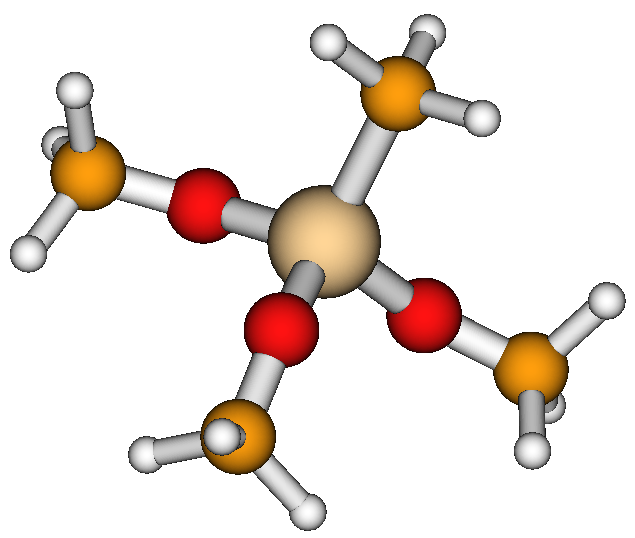
\includegraphics[width=5cm]{si_ch3_och3.png} \label{si_ch3_och3}}
\subfigure[\ce{Si(OCH3)4}, \textbf{B}]{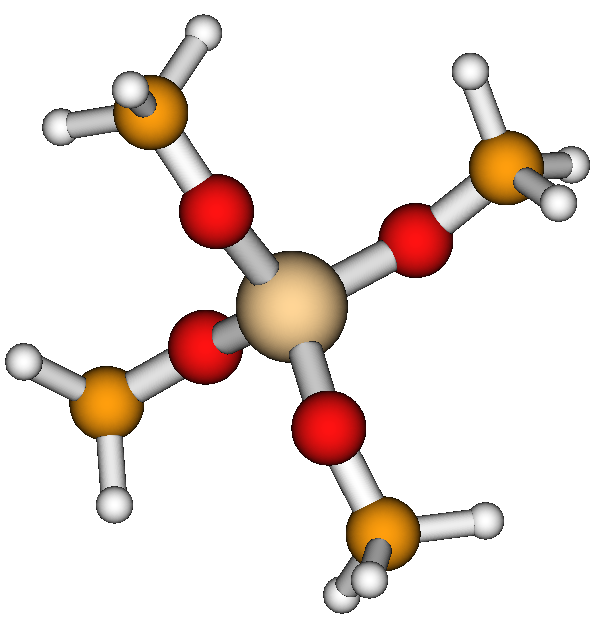
\includegraphics[width=5cm]{si_och3_4.png}\label{si_och3_4}}
\subfigure[\ce{SiCH3(OCH3)5^{2-}},  \textbf{C}]{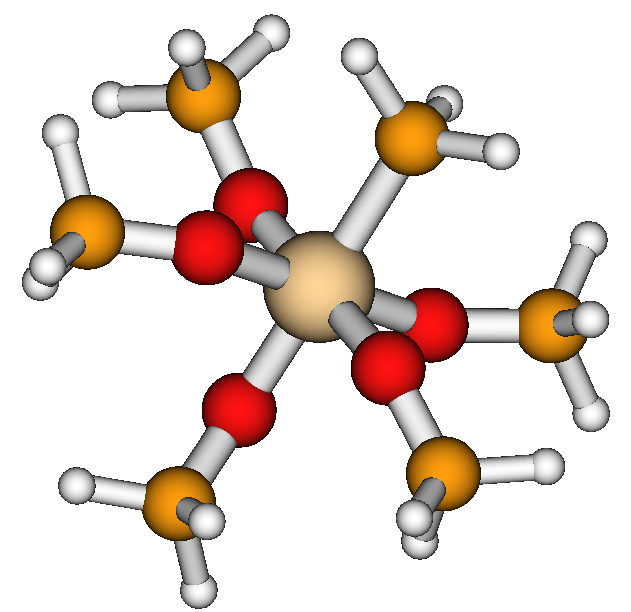
\includegraphics[width=5cm]{si_ch3_och3_5.png}\label{si_ch3_och3_5}}
\subfigure[\ce{Si(OCH3)6^{2-}},  \textbf{D}]{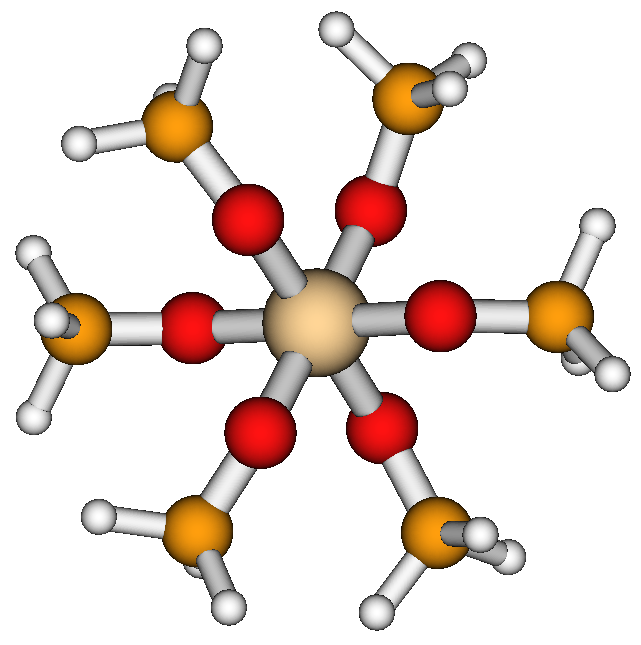
\includegraphics[width=5cm]{si_och3_6.png}\label{si_och3_6}}
\subfigure[\ce{SiCl4},  \textbf{E}]{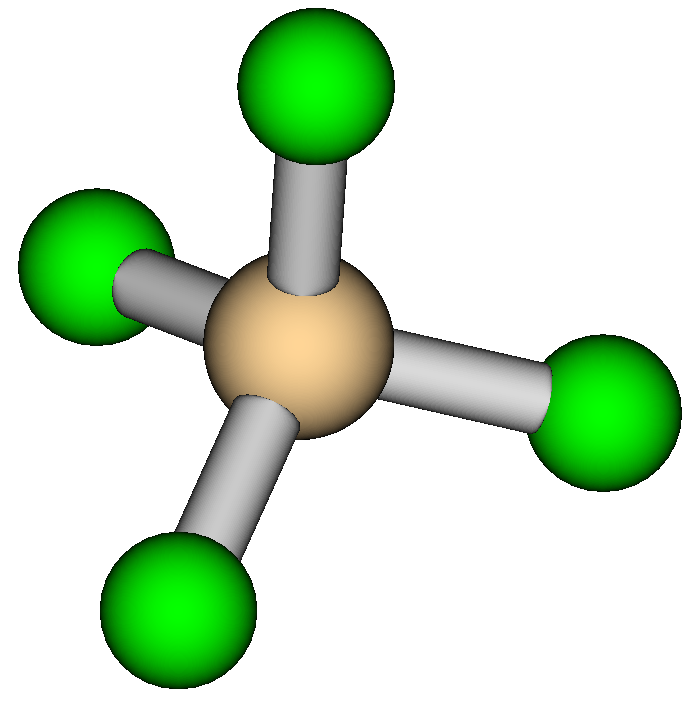
\includegraphics[width=2cm]{si_cl_4.png}\label{si_cl4}}
\subfigure[(acetylmethoxyl)trifluorsilan, \textbf{F}]{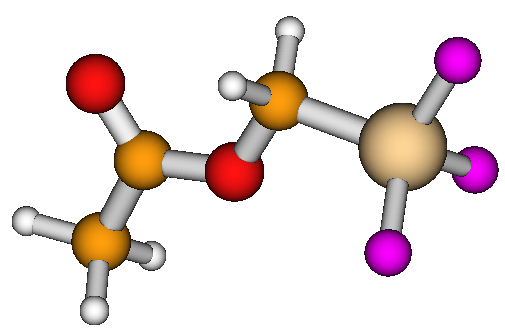
\includegraphics[width=5cm]{acetylmethyltriflurosila.png} \label{acetylmethylfluorsilan}}
\caption{Přehled malých modelů; Legenda: \mycircle{brown} Si, \mycircle{red} O, \mycircle{orange} C, \mycircle{green} Cl, \mycircle{red!50!blue!50}~F, \mycircleempty{black}~H.}
\label{prehled_male_modely}
\end{figure}

Druhou část malých modelů tvořily reaktanty získané například z~práce Aleše Stýskalíka \cite{Styskalik2015thesis}. Struktury reaktantů jsou uvedeny také na obrázku \ref{prehled_male_modely_II}. Tyto struktury obsahovaly křemík v~koordinaci čtyři, který sloužil jako výchozí reaktant pro přípravu silikofosfátových polymerů.

 Struktura \ce{Si(OC2H5)4}, \textbf{G} a~\ce{Si(OCOCH3)4},  \textbf{J}  byly jedny z~výchozích reaktantů pro silikofosfáty v~práci Aleše Stýskalíke \cite{Styskalik2015thesis}. Jedná se o~uspořádání, kdy křemík je ochotný navyšovat koordinaci na šest. Model \ce{SiF3(C6H5)},  \textbf{H} v~práci \cite{aksamentova2009synthesis} byl použit jako prekurzor, ktery také vedl k~navyšování koordinace křemíku. Struktura \ce{Si(OCl)(OC2H5)3}, \textbf{I} zmíněny v~práci \cite{Styskalik2015thesis} také navyšoval koordinaci.

 Jednou z~otázek v~této práci bylo porovnání struktur \ce{Si(OCOCH3)4},  \textbf{J} a~jeho dvou modifikací \ce{SiH(OCOCH3)3},  \textbf{K} a~\ce{SiCH3(OCOCH3)3},  \textbf{L}. Aleš Stýskalík pozoroval, že model \ce{SiH(OCOCH3)3},  \textbf{K} je ochotný navyšovat koordinaci jako prekurzor a~naopak model \ce{SiCH3(OCOCH3)3},  \textbf{L}. Proto byly oba modely zařazeny do této práce.

\begin{figure}
\centering
\subfigure[\ce{Si(OC2H5)4}, \textbf{G}]{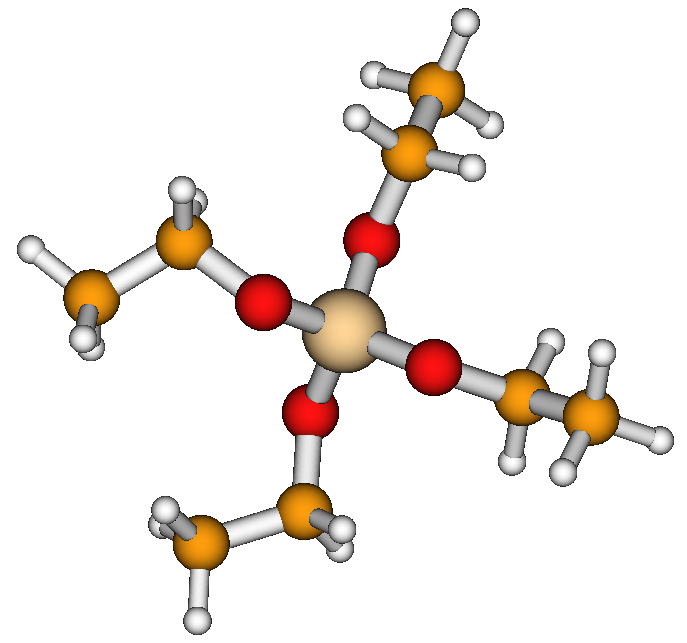
\includegraphics[width=6cm]{si_o_et_4.png} \label{si_oet_4}}
\subfigure[\ce{SiF3(C6H5)},  \textbf{H}]{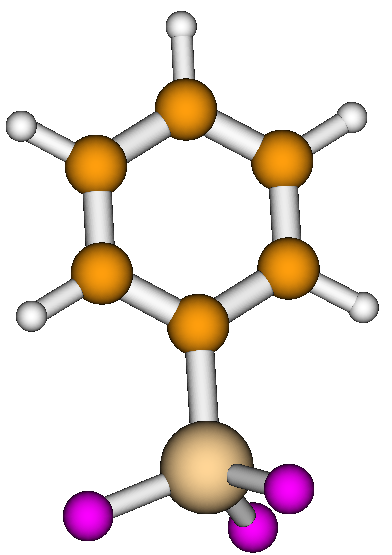
\includegraphics[width=2.5cm]{si_fenyl_f3.png}\label{si_fenyl_f3}}
\subfigure[\ce{Si(OCl)(OC2H5)3},  \textbf{I}]{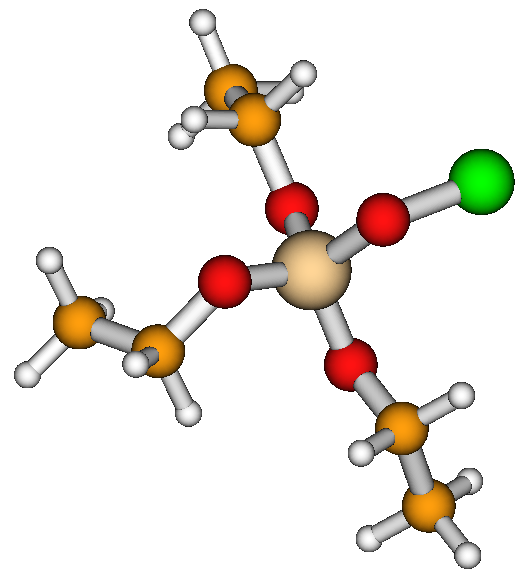
\includegraphics[width=4.5cm]{si_ocl_oet_3.png}\label{si_ocl_oet_3}}
\subfigure[\ce{Si(OCOCH3)4},  \textbf{J}]{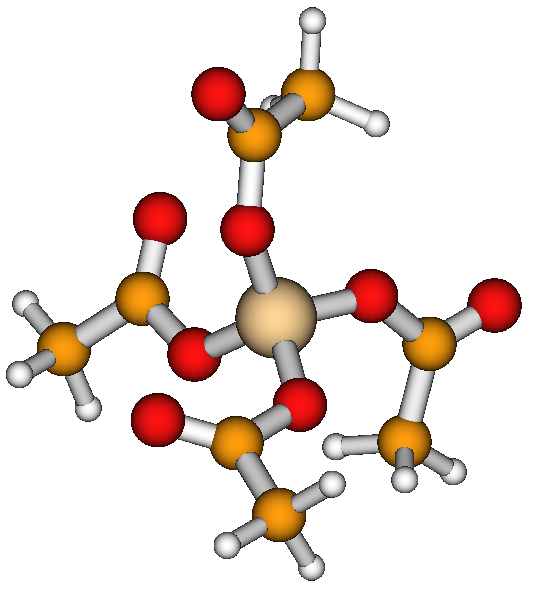
\includegraphics[width=4.5cm]{si_o_ac_4.png}\label{si_o_ac_4}}
\subfigure[\ce{SiH(OCOCH3)3},  \textbf{K}]{\includegraphics[width=4.5cm]{si_h_oac_3.png}\label{si_h_oac_3}}
\subfigure[\ce{SiCH3(OCOCH3)3},  \textbf{L}]{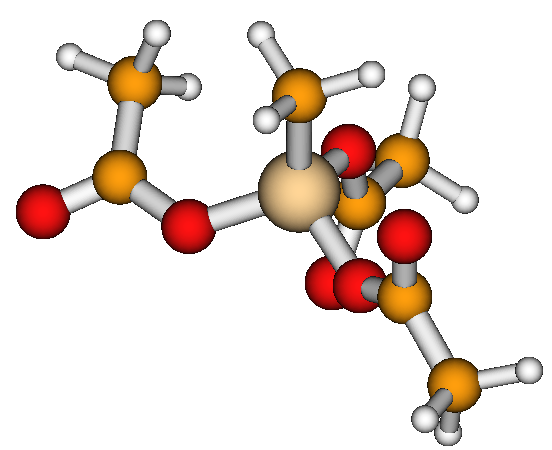
\includegraphics[width=4.5cm]{si_ch3_oac_3.png}\label{si_ch3_oac_3}}
\caption{Přehled struktur, které byly použity pri přípravu silikofosfátů; Legenda: \mycircle{brown} Si, \mycircle{red} O, \mycircle{orange} C, \mycircle{red!50!blue!50} F, \mycircle{green}~Cl, \mycircleempty{black}~H.}
\label{prehled_male_modely_II}
\end{figure}

Pro obě části byla provedena HSAB analýzy. První část výsledků pro modely na obrázku \ref{prehled_male_modely} je uvedena v~tabulce \ref{hsab_small} a~druhá část výsledků pro modely na obrázku \ref{prehled_male_modely_II} je v~tabulce \ref{hsab_small_porovnani}.

Výjimku tvoří dvojice struktur \ce{Si(OCH3)6^{2-}} a~\ce{SiCH3(OCH3)5^{2-}}, které mohou sloužit jako model pro těsné okolí křemíku v~silikofosfátech. Nevýhoda toho malého modelu je ovšem tam, že ligandy nejsou schopny převzít záporný náboj a~hodnoty energii HOMO a~LUMO orbitalu pro tyto systémy jsou nesmyslné. Energie HOMO orbitalu byla přibližně 3 eV a~energie LUMO orbitalu přibližne 9,5 eV. V~tomto případě nemá smysl uvažovat hodnoty tvrdosti ani absolutní elektronegativity. Řešením by byla kompenzace záporného náboje na strukturách, která může být předmětem dalšího výzkumu.

Nejvyšší hodnotu elektronegativity 5,36 eV má model \ce{SiCl4}, \textbf{E} a~je známo, že strukutra \ce{SiCl6^{2-}} nevzniká. Druhou nejvyšší hodnotu elektronegativity 4,81 eV má struktura \ce{Si(OCl)(OC2H5)3}, \textbf{I} v~práci \cite{jahnigen2012synthesis}. Tato struktura již vedla k~vzniku silikofosfátu. Třetí nejvyšší hodnotu 4,16 měly struktury \ce{SiF3(C6H5)},\textbf{H} v~práci \cite{aksamentova2009synthesis} a~\ce{Si(OCOCH3)4}, \textbf{J} v~práci \cite{Styskalik2015thesis}. Obě struktury struktury taktéž vedou ke vzniku silikofosfátu. Struktury (acetylmethoxyl)trifluorsilan,\textbf{F} a~\ce{SiH(OCOCH3)3},\textbf{K} měly hodnotu elektronegativity 3,96 eV a~oba taktéž vedou ke vzniku silikofosfátu. Nejnižší hodnoty elektronegativity vykazovaly struktury \ce{SiCH3(OCH3)3}, \textbf{A}, \ce{Si(OCH3)4}, \textbf{B} a~\ce{Si(OC2H5)4}, \textbf{G} a~to kolem 2,8 eV.

Struktura \textbf{I}, která na sobě nenese výrazně elektronnegativní ligand má vyšší elektronegativity než její modifikovaná analogie \textbf{G}. A~podobná struktura \textbf{A} je hodnotou ještě níže. Struktura \textbf{A} nevede k~navyšování koordinace. Lze tedy říci, že vyšší hodnota elektronegativity vede spíše k~navýšení koordinace.

\begin{table}[H]
\begin{minipage}{\textwidth}
\caption{HSAB analýza molekul z~obrázku \ref{prehled_male_modely}, výsledky jsou uvedeny v~[eV].}
\begin{center}
\begin{tabular}{|l|c|c|c|c|}
\hline
\label{hsab_small}& E$_{\ce{H}}$\footnote{HOMO $-$ \textit{Highest Occupied Molecular Orbital}.}  & E$_{\ce{L}}$\footnote{LUMO$ - $\textit{Lowest Unoccupied Molecular Orbital}.} & $\chi$  & $\eta$  \\ \hline
\ce{SiCH3(OCH3)3}, \textbf{A}& -7,362 & 1,699 & 2,831 & 4,531 \\ \hline
\ce{Si(OCH3)4}, \textbf{B} & -7,389 & 1,442 & 2,974 & 4,416 \\ \hline
%\ce{SiCH3(OCH3)5^{2-}},  \textbf{C} & 3,089 & 10,089 & -6,589 & 3,500 \\ \hline
%\ce{Si(OCH3)6^{2-}},  \textbf{D} & 3,112 & 9,625 & -6,369 & 3,256 \\ \hline
\ce{SiCl4},  \textbf{E} & -9,338 & -1,385 & 5,361 & 3,976 \\ \hline
(acetylmethoxyl)trifluorsilan, \textbf{F} & -7,825 & -0,066 & 3,946 & 3,880 \\ \hline
\end{tabular}
\end{center}
\end{minipage}
\end{table}


\begin{table}[H]\begin{minipage}{\textwidth}
\begin{center}\caption{HSAB analýza malých molekul z~obrázku \ref{prehled_male_modely_II}, výsledky jsou uvedeny v~[eV].}
\begin{tabular}{|l|c|c|c|c|}
\hline
\label{hsab_small_porovnani}& E$_{\ce{H}}$\footnote{HOMO $-$ \textit{Highest Occupied Molecular Orbital}.}  & E$_{\ce{L}}$\footnote{LUMO$ - $\textit{Lowest Unoccupied Molecular Orbital}.} & $\chi$  & $\eta$  \\ \hline
\textbf{G} & -7,181 & 1,662 & 2,760 & 4,422 \\ \hline
\textbf{H} & -7,299 & -1,023 & 4,161 & 3,138 \\ \hline
\textbf{I} & -7,536 & -2,085 & 4,811 & 2,725 \\ \hline
\textbf{J} & -7,669 & -0,642 & 4,155 & 3,513 \\ \hline
\textbf{K} & -7,605 & -0,313 & 3,959 & 3,646 \\ \hline
\textbf{L} & -7,463 & -0,158 & 3,811 & 3,652 \\ \hline
\end{tabular}
\end{center}\end{minipage}
\end{table}

Pro malé modely a~pro reaktany byla provedena NBO analýza. Ta si kladla za cíl lépe popsat vazebné možosti křemíku v~různých koordinacích a~s~různými substituenty. V~NBO analýze byly analyzovány protivazebné orbitaly (BD*). Právě dostupnost BD* určuje, zda bude sloučenina křemíku ochotna navyšovat koordinaci. Model \textbf{A} má dva symetricky ekvivalentní uhlíky (2)O a~(4)O. Jejich obsazovací číslo a~složení se ve výpočtu líší v~řádu $10^{-3}$ (O.Č) a~$10^{-1}$. V~tabulce \ref{nbo_small} uvažujeme aritmetický průměr těchto mírně odlišných čísel. Na základě vysokého podílu křemíku v~BD* u~molekuly \textbf{A} v~tabulce \ref{nbo_small} lze učit, že v~případě vazebných orbitalů (BD) je velká část vazby lokalizována na kyslíku. Pro model \textbf{A} by se jako vhodné místo napojení další vazby pro nárust koordinace jevilo místo  naproti methylu, tedy u~(3)O. Ten se ale řadí mezi objemnější substituenty a~proto zde není možné navýšit koordinaci.

 U~molekuly \textbf{B} lze na hodnotách NBO analý vidět, že je symetrická a~hodnoty pro všechny čtyři vazby mají stejné hodnoty. Navíc se ve BD* vyskytuje menší podíl křemíku a~je zde větší prostor pro nárust koordinace.

Pro šestikoordinované sloučeniny \textbf{C} a~\textbf{D} je podíl křemíku ve vazebných orbitalech velice nízký. Není zde tedy téměř žádný prostor pro další navyšování koordinace. Tyto sloučeniny nebyly ani experimentálně pozorovány. Pro struktury, kde jsou jako ligandy halogenidy  \textbf{E} a~\textbf{F} lze vidět rozdíl v~hodnotách BD*. Jako vyplývá z~experimentu, sloučenina \textbf{F} je schopná navýšit koordinaci na pět a~\textbf{E} nikoliv.

\begin{table}[H]
\begin{minipage}{\textwidth}
\caption{Složení a~obsazovací číslo z~NBO analýzy pro modely z~obrázku \ref{prehled_male_modely}, výsledky jsou uvedeny v~[\%].}
\begin{center}
\begin{tabular}{|l|c|c|c|c|c|c|c|}
\hline
\label{nbo_small} &  Vazba & O.Č\footnote{Obsazovací číslo křemíku.} & Si\footnote{Procentuální příspěvěk křemíku do NBO.} & X\footnote{Procentuální příspěvek atomu vázaného na křemíku do NBO.} & Si(s)\footnote{Rozdělení příspěvku křemíku do orbitálních komponent, součet Si(s) + Si(p) + Si(d) = 100\%.} & Si(p)$^d$ &Si(d)$^d$ \\ \hline
\textbf{A} & (1)Si - O\footnote{ Obsazovací čísla jsou stejná pro vazby (1)Si - (2)O (1)Si - (4)O.}  & 0,066 & 88,4  & 11,6  & 23,8  & 51,1  & 25,2  \\ \hline
&  (1)Si - (3)O\footnote{Lokalizační procedura NBO přiřazuje jednomu atomu (3)O dva vazebné orbitaly.} & 0,111 & 86,5  & 13,5  & 23,2  & 73,3  & 3,5  \\ \hline
&  (1)Si - (3)O$^f$ & 0,092 & 97,1  & 2,9  & 0,2  & 56,7  & 43,3  \\ \hline
& (1)Si - (17)C & 0,073 & 75,5  & 24,5  & 29,3  & 68,9  & 1,8  \\ \hline
\textbf{B} & (1)Si - O\footnote{Obsazovací čísla jsou stejná pro vazby (1)Si-(2)O, (1)Si - (3)O, (1)Si - (4)O a~(1)Si~-~(5)O.}  & 0,104 & 86,1  & 13,9  & 25,0  & 71,4  & 3,6  \\ \hline
\textbf{E} & (1)Si - (2)Cl & 0,141 & 74,0  & 26,0  & 25,0  & 72,4  & 2,6  \\ \hline
&  (1)Si - (3)Cl& 0,141 & 74,0  & 26,0  & 25,0  & 72,4  & 2,6  \\ \hline
& (1)Si - (4)Cl & 0,141 & 74,0  & 26,0  & 25,0  & 72,4  & 2,6  \\ \hline
&  (1)Si - (5)Cl & 0,141 & 74,0  & 26,0  & 25,0  & 72,4  & 2,6  \\ \hline
\textbf{F}  & (1)Si - (2)O &0,107 & 87,1  & 12,9  & 22,5  & 75,6  & 2,0  \\ \hline
& (1)Si - F\footnote{ Obsazovací čísla jsou stejná pro vazby (1)Si - (3)F, (1)Si - (4)F.} & 0,107 & 87,1  & 13,0  & 22,7  & 75,4  & 1,9  \\ \hline
& (1)Si - (5)C &0,079 & 74,3  & 25,7  & 32,2  & 65,8  & 2,0  \\ \hline
\end{tabular}
\end{center}
\end{minipage}
\end{table}

\begin{table}[H]
\caption{Složení a~obsazovací číslo z~NBO analýzy pro modely z~obrázku \ref{prehled_male_modely_II}, výsledky jsou uvedeny v~[\%].}
\begin{minipage}{\textwidth}
\begin{center}
\begin{tabular}{|l|c|c|c|c|c|c|c|}
\hline\label{nbo_reaktanty_porovnani}&  Vazba & O.Č\footnote{Obsazovací číslo křemíku.} & Si\footnote{Procentuální příspěvěk křemíku do NBO.} & X\footnote{Procentuální příspěvek atomu vázaného na křemíku do NBO.} & Si(s)\footnote{Rozdělení příspěvku křemíku do orbitálních komponent, součet Si(s) + Si(p) + Si(d) = 100\%.} & Si(p)$^d$ &Si(d)$^d$ \\ \hline
\textbf{J} & (1)Si-(2)O & 0,096 & 86,3  & 13,7  & 26,0  & 70,9  & 3,1  \\ \hline
& (1)Si-(3)O & 0,128 & 86,5  & 13,5  & 24,5  & 71,9  & 3,6  \\ \hline
& (1)Si-(4)O & 0,101 & 86,3  & 13,7  & 25,4  & 71,4  & 3,1  \\ \hline
& (1)Si-(5)O & 0,103 & 86,7  & 13,3  & 24,1  & 72,6  & 3,2  \\ \hline

\textbf{K} & (1)Si-(2)H & 0,046 & 61,53  & 38,47  & 29,8  & 68,8  & 1,4  \\ \hline
& (1)Si-(3)O & 0,101 & 85,5  & 14,5  & 24,2  & 72,9  & 3,0  \\ \hline
& (1)Si-(4)O & 0,087 & 86,2  & 13,8  & 22,2  & 74,8  & 3,0  \\ \hline
& (1)Si-(5)O & 0,097 & 86,0  & 14,0  & 23,8  & 73,0  & 3,2  \\ \hline
\textbf{L} & (1)C - (2)Si & 0,055 & 73,9  & 26,1  & 32,1  & 66,5  & 1,4  \\ \hline
& (2)Si-(6)O & 0,109 & 86,4  & 13,6  & 23,5  & 73,3  & 3,2  \\ \hline
& (2)Si-(7)O & 0,092 & 86,9  & 13,1  & 21,5  & 75,3  & 3,2  \\ \hline
& (2)Si-(8)O & 0,105 & 86,9  & 13,1  & 22,9  & 73,6  & 3,5  \\ \hline
\end{tabular}
\end{center}\end{minipage}\end{table}

Vizulizace dat z~tabulky \ref{nbo_reaktanty_porovnani} formou obrázků je uvedena na obrázku \ref{prehled_nbo_SI_AC},  \ref{prehled_nbo_SI_H_ac_3} a~\ref{prehled_nbo_si_ch3_oac_3}. Číslování orbitalů se vztahuje k~programu NBO6.

Pro strukturu \ce{Si(OAC)4}, \textbf{J} jsou na obrázku \ref{prehled_nbo_SI_AC} uvedeny obrázky orbitalů BD* č. 70, 71, 72 a~73 s~jejich obsazovacími čísly.Pro strukturu \ce{Si(CH3)(OAC)3}, \textbf{L} jsou na obrázku \ref{prehled_nbo_si_ch3_oac_3} uvedeny orbitaly č. 59, 63, 64, 65 s~jejich obsazovacími čísly. Pro strukturu  \ce{SiH(OCOCH3)3}, \textbf{K} jsou na obrázku \ref{prehled_nbo_SI_H_ac_3} uvedeny obrázky orbitalů č. 30, 31, 32 a~33 s~jejich obsazovacími čísly.
\renewcommand{\thesubfigure}{(\alph{subfigure})}
\begin{figure}
\begin{center}
\caption{Přehled NBO pro \ce{Si(OAC)4}, \textbf{J};  Legenda: \mycircle{black!50!white!50} Si, \mycircle{red} O, \mycircle{black} C, \mycircle{yellow}~P, \mycircleempty{black}~H.}
\subfigure[Si 0,09585]{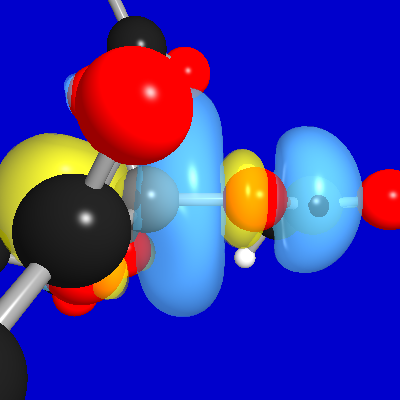
\includegraphics[width=6cm]{SI_AC_70.png} \label{}}
\subfigure[Si 0,12800]{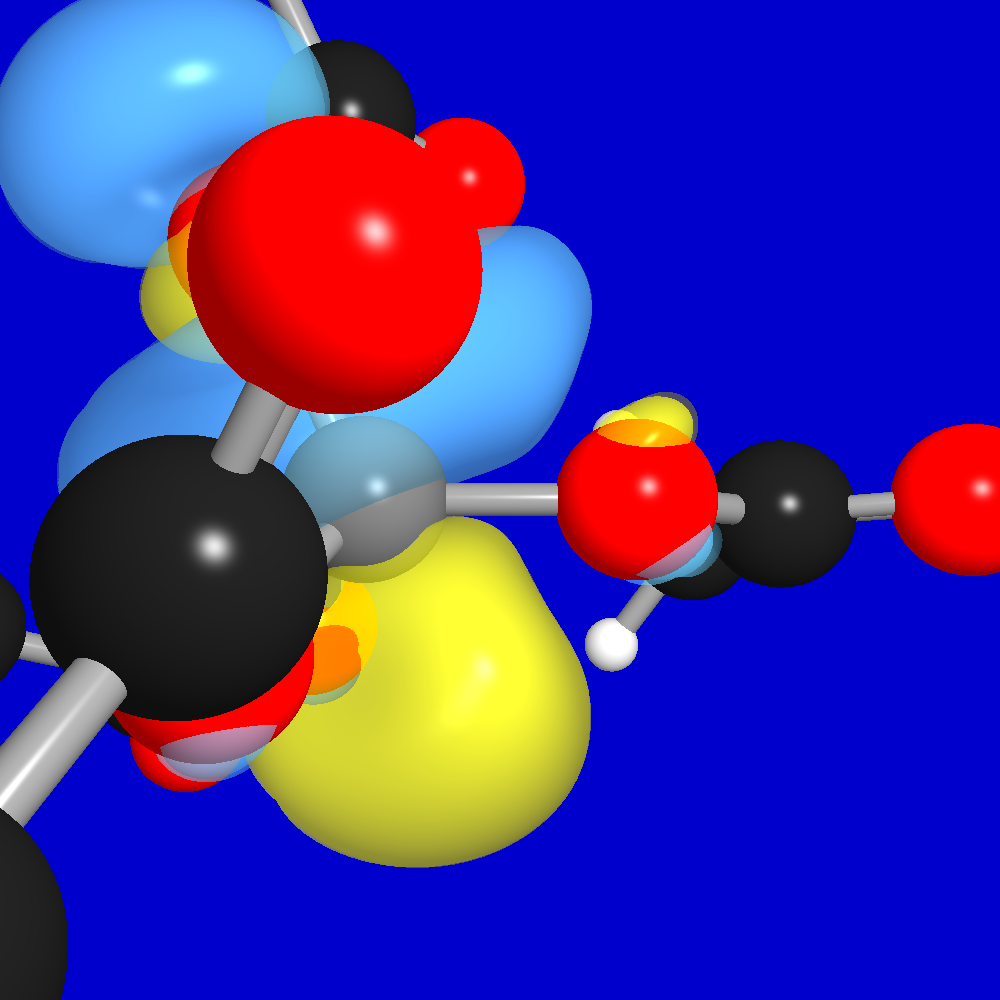
\includegraphics[width=6cm]{SI_AC_71.png}\label{}}
\subfigure[Si 0,10069]{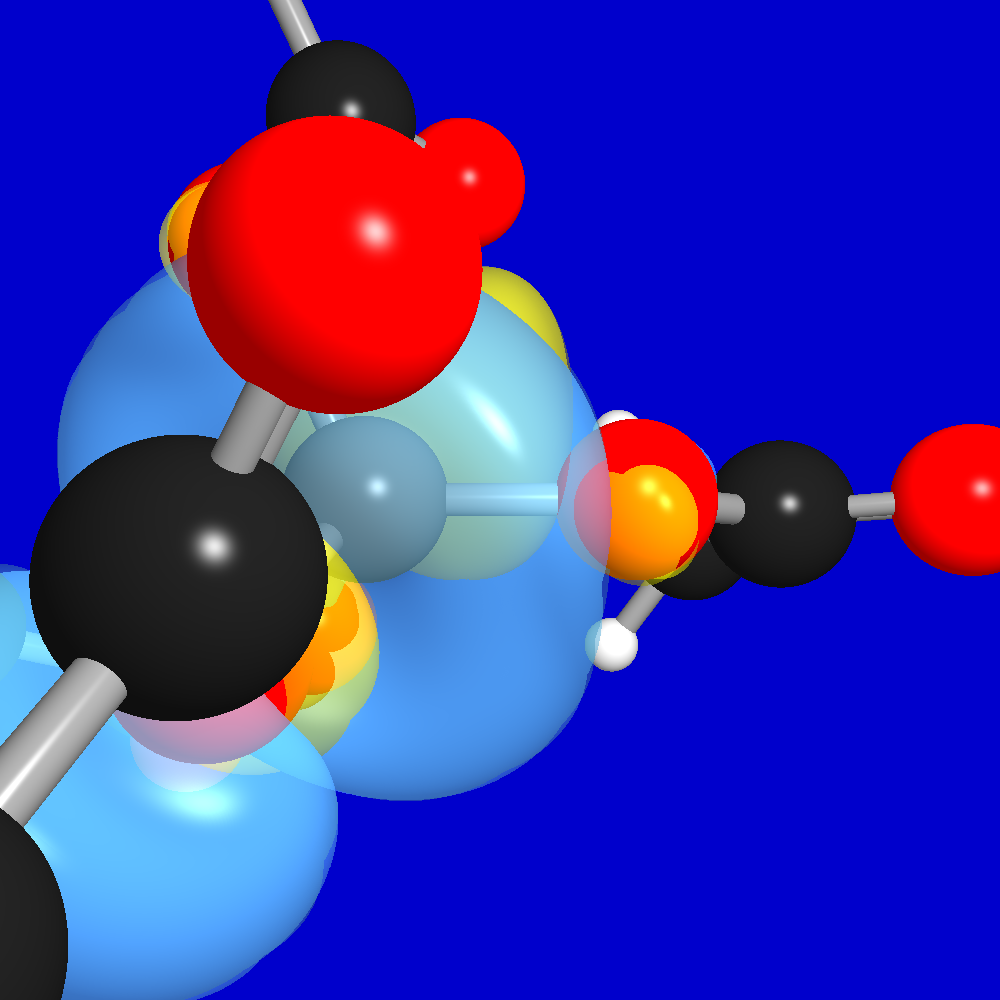
\includegraphics[width=6cm]{SI_AC_72.png}\label{}}
\subfigure[Si 0,10258]{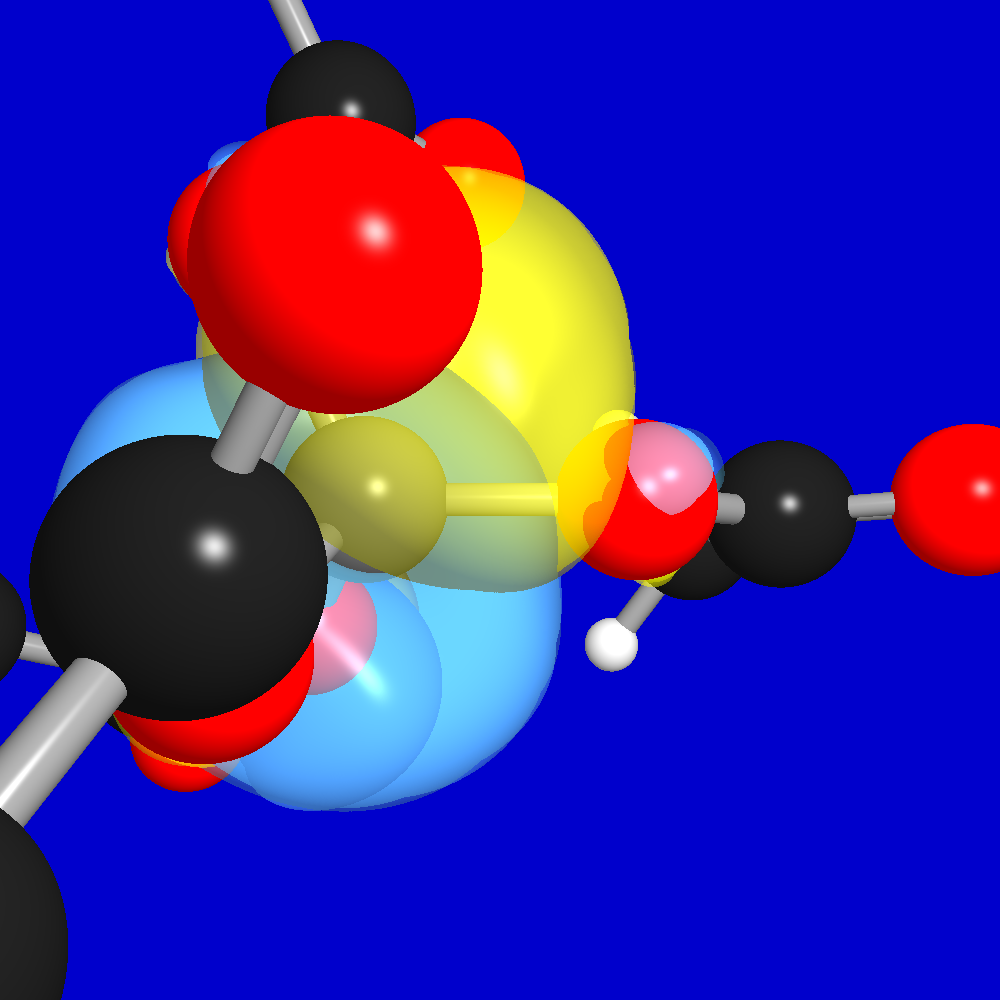
\includegraphics[width=6cm]{SI_AC_73.png}\label{}}
\label{prehled_nbo_SI_AC}
\end{center}
\end{figure}

\begin{figure}
\begin{center}
\caption{Přehled NBO pro \ce{SiH(OCOCH3)3}, \textbf{K};  Legenda: \mycircle{black!50!white!50} Si, \mycircle{red} O, \mycircle{black} C, \mycircle{yellow} P, \mycircleempty{black}~H.}
\subfigure[Si 0,04646]{\includegraphics[width=6cm]{si_h_30.png} \label{}}
\subfigure[Si 0,10132]{\includegraphics[width=6cm]{si_h_31.png}\label{}}
\subfigure[Si 0,08739]{\includegraphics[width=6cm]{si_h_32.png}\label{}}
\subfigure[Si 0,09696]{\includegraphics[width=6cm]{si_h_33.png}\label{}}
\label{prehled_nbo_SI_H_ac_3}
\end{center}
\end{figure}

\begin{figure}
\begin{center}
\caption{Přehled NBO pro \ce{Si(CH3)(OAC)3};  Legenda: \mycircle{black!50!white!50} Si, \mycircle{red} O, \mycircle{black}~C, \mycircle{yellow} P, \mycircleempty{black}~H.}
\subfigure[Si 0,05492]{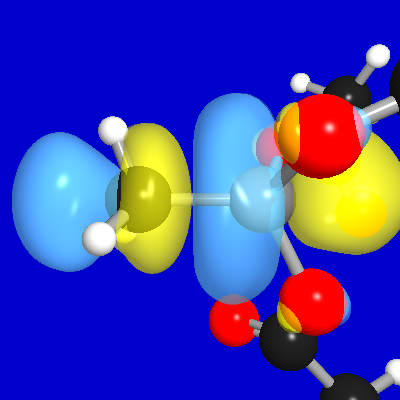
\includegraphics[width=6cm]{si_ch3_59.png} \label{}}
\subfigure[Si 0,10858]{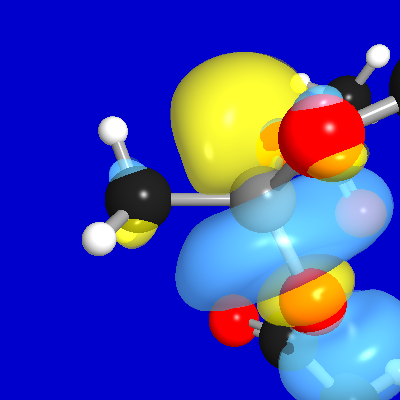
\includegraphics[width=6cm]{si_ch3_63.png}\label{}}
\subfigure[Si 0,09214]{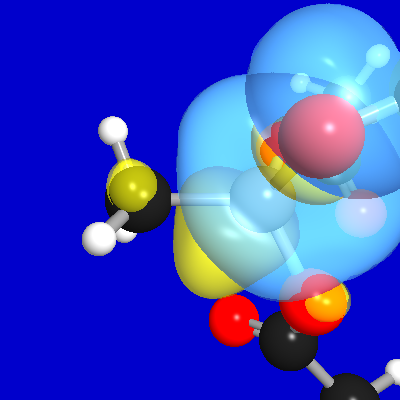
\includegraphics[width=6cm]{si_ch3_64.png}\label{}}
\subfigure[Si 0,10523]{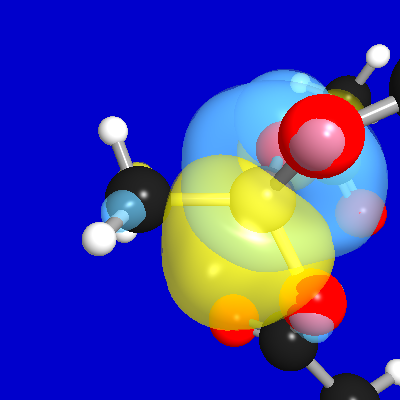
\includegraphics[width=6cm]{si_ch3_65.png}\label{}}
\label{prehled_nbo_si_ch3_oac_3}
\end{center}
\end{figure}

Výsledky MPA pro molekulu \textbf{A} jsou uvedeny v~tabulce \ref{si_ch3_och3_MPA}, pro molekulu \textbf{B} jsou uvedeny v~tabulce \ref{si_och3_4_MPA}, \textbf{C} jsou uvedeny v~tabulce \ref{si_ch3_och3_5_MPA}, \textbf{D} jsou v~tabulce \ref{si_och3_6_MPA}, \textbf{E} jsou v~tabulce \ref{si_cl4} a~\textbf{F} jsou v~tabulce \ref{acetylmethyltrifluorsilan_MPA}. Pro některé molekuly bylo nutno použít vice MO než je počet jejich vazeb kvůli delokalizaci MO přes celou molekulu. Tento případ nastal pro molekuly \textbf{B}, \textbf{C} a~\textbf{D}. Všechny struktury mají nízký podíl křemíku ve vazebných orbitalech, výjimkou je struktura \textbf{E}, kde je procento křemíku asi 43\%. Atomvé orbitaly $3s$ chloru totiž leží pouze 10 eV pod orbitaly $3s$  křemíku a~tvoří proto relativně kovalentní vazby, na rozdíl od dvojice Si-O, kde rozdíl v~polohách orbitalů $s$ činí 17 eV.

\begin{table}[H]\begin{minipage}{\textwidth}
\caption{Mullikenova populační analýza vybraných MO orbitalů pro model \ce{SiCH3(OCH3)3}, \textbf{A}, výsledky jsou uvedeny v~[\%].}
\begin{center}
\begin{tabular}{|l|c|c|c|c|c|}
\hline
Atomy\footnote{Číslo atomu ve výstupu programu Gaussian.} \label{si_ch3_och3_MPA}&  & 20 & 33 & 34 & 35 \\ \hline
(1)Si & s~& 11,8 & 11,8 & 0,2 & 3,2 \\ \hline
& p & 0,2 & 9,7 & 3,0 & 5,4 \\ \hline
(2)O & s~& 2,3 & 2,3 & 0,4 & 26,5 \\ \hline
& p & 9,1 & 17,4 & 26,0 & 34,0 \\ \hline
(3)O & s~& 2,5 & 2,5 & 0,8 & 17,5 \\ \hline
& p & 8,0 & 19,7 & 16,7 & 20,7 \\ \hline
(4)O & s~& 2,2 & 2,2 & 0,4 & 24,7 \\ \hline
& p & 9,0 & 16,5 & 24,3 & 17,1 \\ \hline
(17)C & s~& 1,7 & 1,7 & 0,1 & 1,6 \\ \hline
& p & 4,9 & 2,5 & 1,5 & 1,5 \\ \hline
\end{tabular}
\end{center}
\end{minipage}
\end{table}

\begin{table}[H] \begin{minipage}{\textwidth}
\caption{Mullikenova populační analýza vybraných MO orbitalů pro model \ce{Si(OCH3)4}, \textbf{B}, výsledky jsou uvedeny v~[\%].}
\begin{center}
\begin{tabular}{|l|c|c|c|c|c|c|c|}
\hline
Atomy\footnote{Číslo atomu ve výstupu programu Gaussian.}\label{si_och3_4_MPA} &  & 22 & 23 & 34 & 35 & 36 & 37 \\ \hline
(1)Si & s~& 11,1  & 0,0  & 4,6  & 0,0  & 0,0  & 0,0  \\ \hline
& p & 0,0  & 5,1  & 0,0  & 12,3  & 12,3  & 2,7  \\ \hline
(2)O& s~& 2,5  & 0,0  & 3,1  & 1,7  & 3,8  & 0,2  \\ \hline
& p & 5,4  & 6,5  & 9,0  & 9,4  & 9,3  & 15,4  \\ \hline
(3)O & s~& 2,5  & 0,0  & 3,1  & 3,8  & 1,7  & 0,2  \\ \hline
& p & 5,4  & 3,3  & 4,5  & 9,3  & 9,4  & 15,4  \\ \hline
(4)O & s~& 2,5  & 0,0  & 3,1  & 1,7  & 3,8  & 0,2  \\ \hline
& p & 5,4  & 3,3  & 4,5  & 9,4  & 9,3  & 15,4  \\ \hline
(5)O & s~& 2,5  & 0,0  & 3,1  & 3,8  & 1,7  & 0,2  \\ \hline
& p & 5,4  & 3,3  & 4,5  & 9,3  & 9,4  & 15,4  \\ \hline
\end{tabular}
\end{center}
\end{minipage}
\end{table}

\begin{table}[H] \begin{minipage}{\textwidth}
\begin{center}
\caption{Mullikenova populační analýza vybraných MO orbitalů pro model \ce{SiCl4}, \textbf{E}, výsledky jsou uvedeny v~[\%].}
\begin{tabular}{|l|c|c|c|c|c|}
\hline
Atomy\footnote{Číslo atomu ve výstupu programu Gaussian.} \label{MP_si_cl4} &  & 30 & 31 & 32 & 33 \\ \hline
(1)Si & s~& 42,5  & 0,0  & 0,0  & 0,0  \\ \hline
& p & 0,0  & 18,5  & 18,5  & 18,5  \\ \hline
(2)Cl & s~& 12,0  & 0,3  & 3,5  & 7,2  \\ \hline
& p & 5,5  & 5,7  & 12,8  & 20,7  \\ \hline
(3)Cl & s~& 12,0  & 8,9  & 2,0  & 0,1  \\ \hline
& p & 5,5  & 24,5  & 9,5  & 5,2  \\ \hline
(4)Cl & s~& 12,0  & 0,0  & 3,6  & 7,4  \\ \hline
& p & 5,5  & 5,1  & 12,8  & 21,2  \\ \hline
(5)Cl & s~& 12,0  & 5,5  & 5,5  & 0,0  \\ \hline
& p & 5,5  & 16,9  & 17,0  & 5,1  \\ \hline
\end{tabular}\end{center}\end{minipage}\end{table}


\begin{table}[H] \begin{minipage}{\textwidth}
\caption{Mullikenova populační analýza vybraných MO orbitalů pro model acetylmethyltrifluorsilanu, \textbf{F}, výsledky jsou uvedeny v~[\%].}
\begin{center}
\begin{tabular}{|l|c|c|c|c|c|}
\hline
Atomy\footnote{Číslo atomu ve výstupu programu Gaussian.}\label{acetylmethyltrifluorsilan_MPA}&  & 22 & 25 & 26 & 27 \\ \hline
(1)Si & s~& 17,9  & 0,3  & 6,9  & 0,9  \\ \hline
& p & 0,2  & 8,9  & 0,9  & 7,5  \\ \hline
(2)O & s~& 4,3  & 3,4  & 6,7  & 1,9  \\ \hline
& p & 9,0  & 22,2  & 1,9  & 13,6  \\ \hline
(3)O & s~& 5,4  & 1,5  & 19,6  & 0,1  \\ \hline
& p & 9,9  & 12,6  & 0,1  & 6,8  \\ \hline
(4)O & s~& 5,4  & 1,5  & 19,6  & 0,1  \\ \hline
& p & 9,9  & 12,6  & 0,1  & 6,8  \\ \hline
(5)C & s~& 2,6  & 0,9  & 0,5  & 0,7  \\ \hline
& p & 4,9  & 0,9  & 0,7  & 1,8  \\ \hline
\end{tabular}\end{center}\end{minipage}\end{table}



\section{Středně velké modely}
Modely střední velikosti reprezentovaly širší okolí křemíku \ref{prehled_middle} a~už obsahovaly cykly, prozatím bez síťování, které je pro silikofosfáty typické. \\
Model \ce{SiCH3(PO4)CH3(SiP2O10)(CH3)4} obsahoval jeden cyklus, volně navázaný fosfát a~přímou vazbu křemík-uhlík. Model \ce{Si(P2SiO10(CH3)4)2} už obsahoval dva cykly, které byly pozorovány v~silikofosfátových polymerech. Jednalo se o~nejmenší model, který už obsahoval dva cykly.\\
Tato část se věňuje nejmenším možným modelům, které již tvoří uvnitř svých struktur cyklus. Přehled struktur je ukázán na obrázku \ref{prehled_middle}. Středně velké modely obsahují křemík v~koordinaci čtyři a~snaží se zachytiti tvorbu cyklů, které jsou pozorovány v~silikofosfátech.
\begin{figure}
\begin{center}
\subfigure[\ce{SiCH3(PO4(CH3)2)(Si2P2O9(CH3)4)},  \textbf{M}]{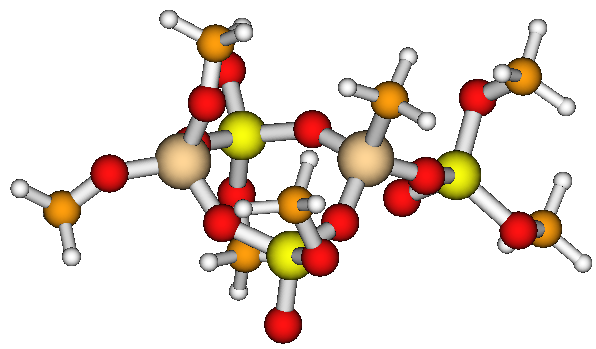
\includegraphics[width=6cm]{si_model_methyl.png}\label{obr_h4sio4_MO_s1_20}}
\subfigure[\ce{Si(Si2P2O9(CH3)4)2}, \textbf{N}]{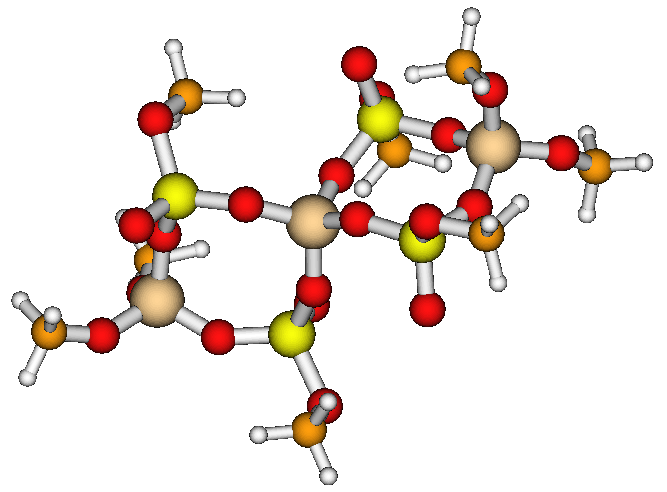
\includegraphics[width=5cm]{si_model_orezany.png}\label{obr_h4sio4_MO_s1_24}}
\caption{Přehled středně velkých modelů];  Legenda: \mycircle{brown} Si, \mycircle{red} O, \mycircle{orange}~C, \mycircle{yellow} P, \mycircleempty{black}~H.}
\label{prehled_middle}
\end{center}
\end{figure}
V~tabulce \ref{hsab_middle} lze vidět výsledky pro HSAB analýzu. Z~výsledku je vidět podobná hodnota $\eta$, tedy podobná globální tvrdost.

\begin{table}[H]
\begin{minipage}{\textwidth}
\caption{HSAB analýza středních molekul, výsledky jsou uvedeny v~[eV].}
\begin{center}
\begin{tabular}{|l|r|r|r|r|}
\hline
\label{hsab_middle}& E$_{\ce{H}}$\footnote{HOMO $-$ \textit{Highest Occupied Molecular Orbital}.}  & E$_{\ce{L}}$\footnote{LUMO$ - $\textit{Lowest Unoccupied Molecular Orbital}.} & $\chi$  & $\eta$ \\ \hline
\textbf{M} & -7,802 & 0,494 & 3,654 & 4,148 \\ \hline
\textbf{N} & -8,101 & -0,059 & 4,080 & 4,021 \\ \hline
\end{tabular}
\end{center}
\end{minipage}
\end{table}

U~středně velkých modelů bylo cílem ověřit, zda trendy $\chi$ a~kovalenci/ionicite jednotlivých vazeb nalezené u~modelů malých platí i při rozšíření modelu a~přidání cyklů do struktur. V~tomto případě lze porovnávat dvojice struktur \textbf{M}, \textbf{N} a~\textbf{J} a~\textbf{L}. Hodnoty elektronegativity pro střední modely z~obrázku \ref{prehled_middle} jsou v~tabulce \ref{hsab_middle}. Lze zde pozorovat trend, že rozdíl elektronegativity mezi modelem \textbf{J} a~\textbf{N} je velice podobnýjaok rozdíl elektronegativit pro \textbf{L} a~\textbf{M}. Lze tedy říci, že použití malých modelů bez cyklů také vede ke správným trendům.

Výsledky analýzy NBO jsou uvedeny v~tabulce \ref{nbo_middle}. Pro strukturu \textbf{M} lze vidět menší zapojení uhlíku do orbitalů BD*, tedy větší zapojení do vazebných orbitalů. Oproti tomu model \textbf{N} má podobná procenta křemíku v~protivazebných orbitalech.

\begin{table}[H]
\begin{minipage}{\textwidth}
\caption{Složení a~obsazovací číslo z~NBO analýzy pro modely z~obrázku \ref{prehled_middle}, výsledky jsou uvedeny v~[\%].}
\begin{tabular}{|l|c|c|c|c|c|c|c|}
\hline
\label{nbo_middle} &  Vazba & O.Č\footnote{Obsazovací číslo křemíku.} & Si\footnote{Procentuální příspěvěk křemíku do NBO.} & X\footnote{Procentuální příspěvek atomu vázaného na křemíku do NBO.} & Si(s)\footnote{Rozdělení příspěvku křemíku do orbitálních komponent, součet Si(s) + Si(p) + Si(d) = 100\%.} & Si(p)$^d$ &Si(d)$^d$ \\ \hline
\textbf{M} & (1)Si - (2)O & 0,087 & 87,5  & 12,5  & 23,8  & 73,1  & 3,1  \\ \hline
& (1)Si - (3)O & 0,093 & 87,3  & 12,7  & 23,0  & 73,5  & 3,6  \\ \hline
&(1)Si - (4)O & 0,094 & 87,5  & 12,5  & 22,6  & 73,9  & 3,4  \\ \hline
& (1)Si - (5)C & 0,065 & 74,1  & 25,9  & 30,7  & 67,7  & 1,6  \\ \hline
\textbf{N} & (1)Si - (2)O & 0,086 & 87,1  & 12,9  & 25,7  & 71,1  & 3,3  \\ \hline
& (1)Si - (3)O & 0,104 & 87,4  & 12,6  & 23,9  & 72,5  & 3,6  \\ \hline
& (1)Si - (4)O & 0,098 & 87,2  & 12,8  & 24,6  & 71,9  & 3,5  \\ \hline
& (1)Si - (5)O & 0,092 & 86,8  & 13,2  & 25,8  & 70,8  & 3,4  \\ \hline
\end{tabular}
\end{minipage}
\end{table}


Pro středně velké modely byla provedna MPA. Vzhledem k~existenci cyklů bylo nutno pro popis vazeb vybrat více MO než je počet vazeb ve strutkurách. Pro strukturu \textbf{M} jsou výsledky uvedeny v~tabulce \ref{si_model_methyl_MPA_I}. Z~hodnot pro MO 61 lze vidět zapojení uhlíku do vazby. Ve struktuře \textbf{N}, která již obsahuje cyklus, vzrostla hodnota $\chi$.

\begin{table}[H]\begin{minipage}{\textwidth}
\caption{Mullikenova populační analýza vybraných MO orbitalů pro model \ce{SiCH3(PO4(CH3)2)(Si2P2O9(CH3)4)}, \textbf{M}, výsledky jsou uvedeny v~[\%].}
\begin{center}
\begin{tabular}{|l|c|c|c|c|c|c|c|c|c|c|}
\hline
Atomy\footnote{Číslo atomu ve výstupu programu Gaussian.}   \label{si_model_methyl_MPA_I}  &  & 61 & 68 & 69 & 70 & 71 & 72 & 96 & 97 & 106 \\ \hline
(1)Si  & s~& 3,8  & 4,4 &  0,1  & 3,9  & 0,3  & 0,0  & 0,6  & 1,7  & 1,0  \\ \hline
& p & 0,1  & 0,4& 1,6  & 0,5  & 2,4  & 2,0  & 3,2  & 1,3  & 1,2  \\ \hline
(2)O & s~& 0,0  & 0,2& 0,1  & 0,1  & 2,3  & 0,3  & 0,3  & 4,3  & 0,6  \\ \hline
& p & 2,2  & 2,4& 0,2  & 12,4  & 13,0  & 0,4  & 10,6  & 17,8  & 4,5  \\ \hline
(3)O & s~& 0,1  & 0,1& 2,5  & 0,2  & 0,0  & 0,3  & 0,2  & 1,5  & 0,0  \\ \hline
& p & 1,7  & 6,5 &7,2  & 3,4  & 7,1  & 13,8  & 1,4  & 1,3  & 13,4  \\ \hline
(4)O & s~& 0,0  & 0,2& 1,5  & 0,8  & 0,3  & 0,3  & 0,5  & 0,1  & 0,0  \\ \hline
& p & 2,5  & 7,8& 10,5  & 0,8  & 7,6  & 10,0  & 0,2  & 1,6  & 13,7  \\ \hline
(40)C & s~& 19,7  & 6,7& 0,1  & 1,8  & 0,1  & 0,0  & 0,0  & 0,1  & 3,0  \\ \hline
& p & 0,1  & 0,2& 0,1  & 0,3  & 0,1  & 0,1  & 5,0  & 7,3  & 4,4  \\ \hline
\end{tabular}
\end{center}\end{minipage}\end{table}

Výsledky MPA pro strukturu \textbf{N} jsou uvedeny v~tabulce \ref{si_model_orezany_MPA}. Vzhledem k~přítomností cyklů bylo nutno pro popis použít vice MO, než je skutečný počet vazeb ve struktuře. Z~výsledky v~tabulce \ref{si_model_orezany_MPA} lze vidět, že všechny MO mají podobné rozložení. Což odpovídá relativně symetrické podobě modelu \textbf{N}.

\begin{table}[H]\begin{minipage}{\textwidth}
\caption{Mullikenova populační analýza vybraných MO orbitalů pro model \ce{Si(Si2P2O9(CH3)4)2}, \textbf{N},výsledky jsou uvedeny v~[\%].}
\begin{center}
\begin{tabular}{|l|c|c|c|c|c|c|c|}
\hline
Atomy\footnote{Číslo atomu ve výstupu programu Gaussian.}  \label{si_model_orezany_MPA} &  & 99 & 97 & 95 & 94 & 90 & 68 \\ \hline
(1)Si & S~& 0,2  & 0,1  & 0,0  & 0,6  & 48,1  & 2,2  \\ \hline
& P & 1,6  & 2,7  & 1,8  & 0,3  & 6,7  & 0,0  \\ \hline
(2)O & S~& 0,0  & 0,8  & 0,1  & 0,6  & 0,4  & 0,6  \\ \hline
& P & 0,4  & 5,2  & 3,6  & 5,2  & 4,1  & 0,5  \\ \hline
(3)O & S~& 0,1  & 3,3  & 0,8  & 2,3  & 1,4  & 1,1  \\ \hline
& P & 0,3  & 1,4  & 2,7  & 2,3  & 2,3  & 9,5  \\ \hline
(4)O & S~& 0,1  & 2,4  & 0,7  & 1,5  & 1,8  & 0,8  \\ \hline
& P & 5,1  & 2,5  & 5,5  & 3,8  & 2,6  & 7,7  \\ \hline
(5)O & S~& 4,3  & 1,2  & 2,3  & 2,4  & 1,0  & 0,3  \\ \hline
& P & 7,4  & 7,2  & 4,2  & 3,4  & 4,5  & 6,6 \\ \hline
\end{tabular}
\end{center}\end{minipage}\end{table}


\section{Velké modely}
Poslední část, velké modely, se soustřeďují na sloučeniny pěti a~šestikoordinovaného křemíku, obsahující dva a~více cyklů. Naším cílem bylo vytvořit strukturní modely silikofosfátů optimalizací geometrie zkušebních modelech a~validovat je na základě porovnání teoreticky vypočtených chemických posunů křemíku s~experiment. Velké modely měly za cíl modelovat vybrané části ze silikofosfátů. Ve svých strukturách už obsahují dva a~více cyklů a~všechny obsahují křemík v~koordinaci pět nebo šest. Zde je klíčové zmínit, že naše modely byly pouze výseky z~rozsáhlých struktur polymerů a~chyběla stabilizace okolními atomy. Při tvorbě našich tzv. klastrových modelů se ukázala být klíčovou otázka nasycení koncových vazeb a~souvisejícího náboje klastrů. Na rozdíl od hlinitokřemičitanů (tzv. zeolitů), jejichž skelety jsou typicky aniontové a~které ve svých pórech obsahují kompenzující kationty, jsou struktury silikofosfátů neutrální. Proto jsme velke modely tvořili jako elektricky neutrální se dvěma výjimkami. První výjimkou byl model původní retngenové struktury z~práce \cite{C3NJ00721A}(obrázek \ref{rtg_koordinace_sest}), která byla připravena jako aniont. Pro menší výpočetní náročnost byly u~tohoto modelu nahrazeny okolní ethyly za methyly. Struktura byla označena jako \textbf{O}. Již upravená struktura s~methyly je uvedena na obrázku \ref{prehled_large}. Druhou výjimkou tvoří model silikofosfátu s~pětikoordinovaným křemíkem \textbf{S} na obrázku \ref{prehled_largeI}. V~ostatních struktury byly zachovány jako neutrální.

Strutkura \textbf{P} představuje model původní struktury získané z~rentgenové krystalografie, ale již s~neutrálním nábojem. Schéma struktury \textbf{P} je na obrázku \ref{schema_fosfat}.
\begin{figure}\begin{center}\includegraphics[width=7cm]{schema_fosfat_1.eps}
\caption{Schematické znázornění modelu \textbf{P}}\label{schema_fosfat}
\end{center}\end{figure}
Původní rentgenová srtuktura silikofosfátu \ref{rtg_koordinace_sest}, modifikována na struktur \textbf{P} byla zároveň výchozí strukturou pro všechny velké modely silikofosfátů v~koordinaci šest na obrázku  \ref{prehled_large}. V~modelu \textbf{P} je křemík obklopen šesti fosfáty, které jsou vzájemně zesíťované přes další čtyřkoordinované křemíky. Přítomnost osmičlenného cyklu v~silikofosfátech byla potvrzena rentgenovou strukturou \ref{rtg_4} ve článku \cite{rtg_4_pinkas}, která sloužila jako motiv pro vytváření cyklů v~silikofofátových polymerech.
\begin{figure}
\begin{center}
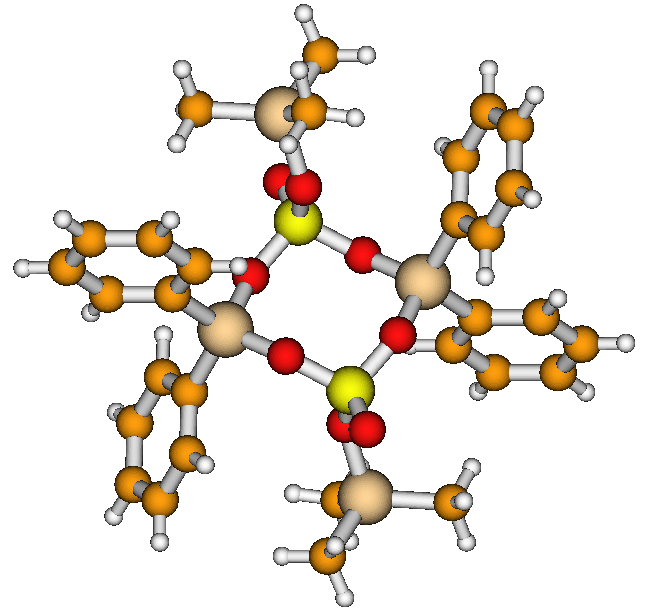
\includegraphics[width=7cm]{rtg_4_kruh_samotne.png}
\caption{Struktura \ce{[(Ph2Si{O2P(O)OSiMe3})2]} získaná pomocí rentgenové krystalografie v~práci \cite{rtg_4_pinkas};  Legenda: \mycircle{brown} Si, \mycircle{red} O, \mycircle{orange} C, \mycircleempty{black}~H.}
\label{rtg_4}
\end{center}
\end{figure}
\\

V~experimentálních strukturách silikofosfátů byly pozorovány krom fosfátových skupiny také acetátové skupiny. Právě přítomnost acetátových skupin měla vliv na chování křemíku a~jeho sklon k~hypervalenci. Acetátové skupiny se  v~okolí křemíku vždy vyskytovaly po dvou a~tento jev byl dodržen i v~modelových strukturách. Zvolila jsem dvě možnosti umístění acetátů. Při modelování silikofosfátů s~acetátovými skupinami v~polohách cis a~trans jsme vycházeli z~uspořádání v~původní rentgenové struktuře. V~prvním případě se acetylové skupiny vůči sobě vyskytovaly v~poloze trans, viz. struktura \textbf{R} na obrázku \ref{prehled_largeI}. Schéma struktury \textbf{R} je uvedeno na obrázku \ref{schema_fosfat_trans}. Ve druhém případě se acetáty vysvytovaly v~poloze cis, viz. struktura \textbf{Q} na obrázku \ref{prehled_largeI}. Schéma struktury \textbf{Q} je uvedeno na obrázku \ref{schema_fosfat_cis}.
\begin{figure}\begin{center}\includegraphics[width=7cm]{struktrua_c_trans_1.eps}
\caption{Schématické znázornění modelu \textbf{R}}\label{schema_fosfat_trans}
\end{center}\end{figure}

\begin{figure}\begin{center}\includegraphics[width=8cm]{struktrua_c_trans_1.eps}
\caption{Schématické znázornění modelu \textbf{Q}}\label{schema_fosfat_cis}
\end{center}\end{figure}
\begin{figure}\begin{center}
\caption{Model motivovaný strukturou získanou z~rentgenové krystalografie v~práci \cite{C3NJ00721A};  Legenda: \mycircle{brown} Si, \mycircle{red} O, \mycircle{orange} C, \mycircle{yellow} P, \mycircleempty{black}~H.}
\subfigure[ \textbf{O}]{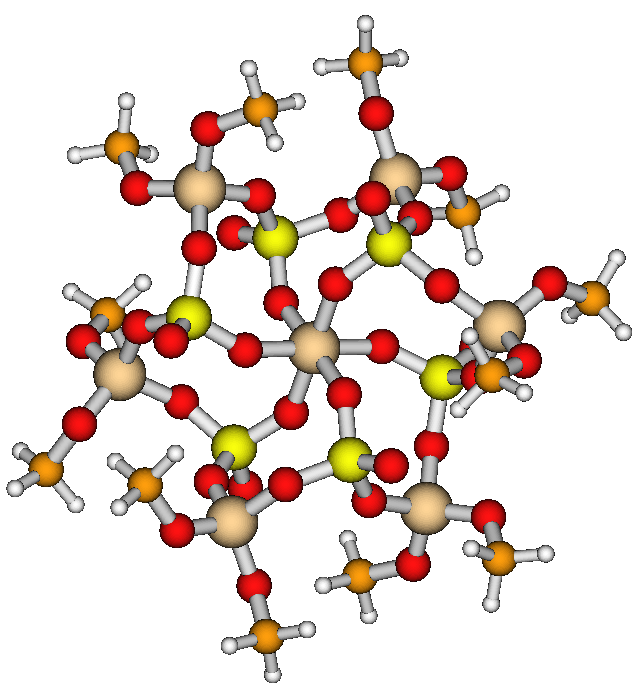
\includegraphics[width=6cm]{struktura_puvodni.png}\label{struktura_puvodni}}
\subfigure[ \textbf{P}]{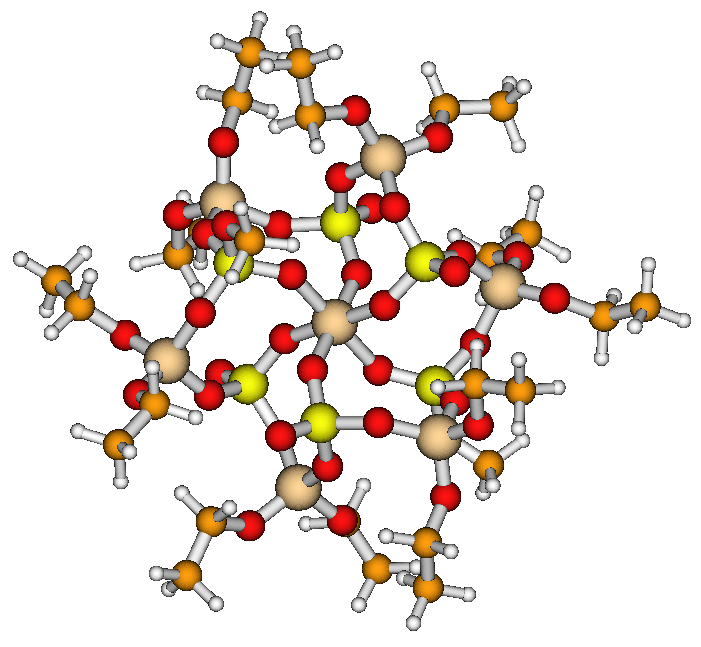
\includegraphics[width=6cm]{srtuktura_bez_naboje.png}\label{struktura_bez_naboje}}
\label{prehled_large}\end{center}
\end{figure}

Při modelování struktur \textbf{Q} a~\textbf{R} bylo snahou zachovat původních šest cyklů. Proto v~prvním kole optimalizace struktury s~acetáty v~poloze trans bylo ponecháno šest cyklů a~dvě fosfátové skupiny nahrazeny acetátovými.

Optimalizace tohoto modelu byla algoritmem ukončena, aniž by dosáhla stacionárního bodu, díky příliš velké hodnotě vazebného úhlu na jednom z~atomů kyslík. Úheů 50-11-52 dosahoval hodnoty 180$^\circ$. V~literatuře tento úhle dosahuje hodnot 134$^\circ$ až 150$^\circ$, maximální hodnota je 160$^\circ$ \cite{yuan2003si}. Příliš vysokou hodnotu měly i torzní úhly na atomech kyslíku. %52 - 11 - 50 - 51 a~50 - 11 - 52 - 54.
Jako řešení situace jsme zvolili odstranění dvou cyklů ze struktury. Rozpojení cyklů bylo realizováno odstraněním protilehlých čtyřkoordinovaných křemmíků, které vytvářely cyklus. Díky tomu došlo k~uvolnění napětí na jednotlivých cyklech. Počet cyklů dva byl zvolen z~důvodu zachování symetrie. Uvolněná struktura silikofosfátu s~acetáty v~poloze trans byla opět optimalizována, tentokrát s~pseudopotenciálem z~důvodu velikosti struktury. Ve druhém kroku byla provedena optimalizace již s~B3LYP/6-31G*. Struktura je schematicky zobrazena na obrázku \ref{schema_fosfat_trans}.\\

\begin{figure}
\begin{center}
\caption{Přehled velkých modelů;  Legenda: \mycircle{brown} Si, \mycircle{red} O, \mycircle{orange} C, \mycircle{yellow} P, \mycircleempty{black}~H.}
\subfigure[ \textbf{Q}]{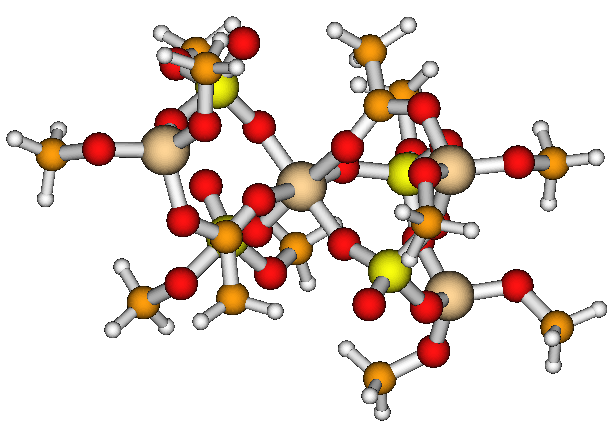
\includegraphics[width=6cm]{struktura_cis.png} \label{struktura_cis}}
\subfigure[ \textbf{R}]{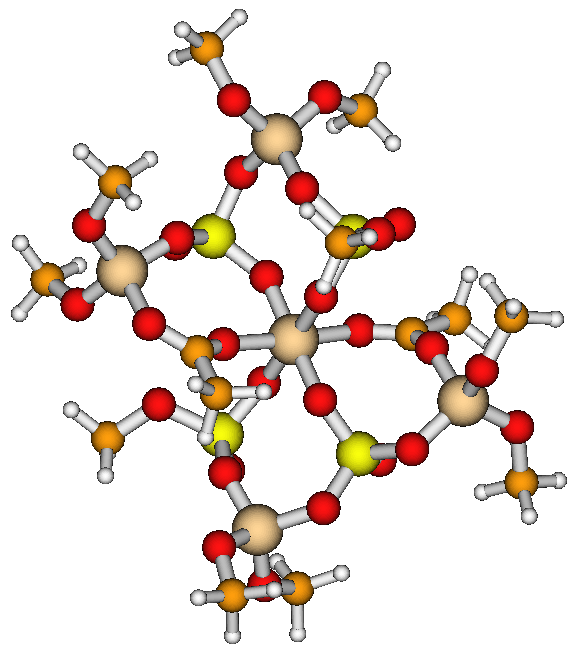
\includegraphics[width=6cm]{struktura_trans.png}\label{struktura_trans}}
\subfigure[ \textbf{S}]{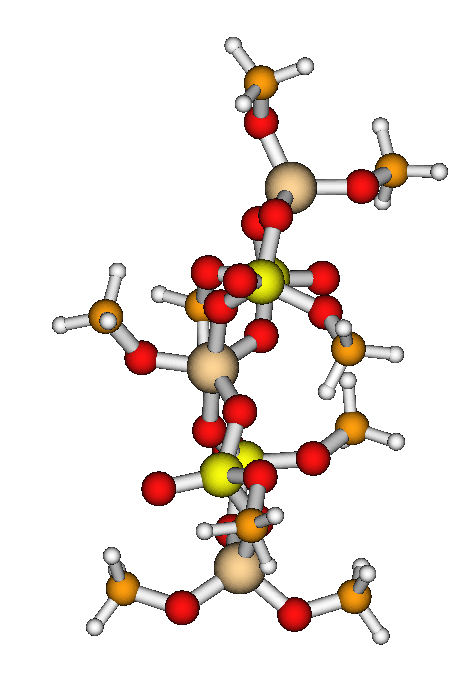
\includegraphics[width=6cm]{strukutra_5_opravena.png}\label{struktura_5}}
\label{prehled_largeI}
\end{center}
\end{figure}
Pro model silikofosfátu s~acetáty v~poloze cis byla situace obdobná. Toto uspořádání opět vedlo k~přílišnému napětí na cyklech a~z~tohoto důvodu byla provedena stejná operace, jako pro model s~acetátem v~poloze trans. Odstranění protilehlých čtyřkoordinovaných křemíků, které vytvářely cyklus. V~modelu silikofofátu s~acetátem v~poloze cis byly odstraněny nejprve dva cykly a~následně ještě jeden, protože struktura stále vykazovala špatné torzní úhly.
Pro strukturu s~acetátem v~poloze cis bylo nutno odstranit celkově čtyři cykly a~výsledný počet cyklů v~molekule byl dva. Acetáty byly umístěné v~ekvatoriální rovině stejně jako volný fosfát. Struktura je schematicky znázorněna na obrázku \ref{schema_fosfat_cis}. \\


Další koordinace křemíku, která byla experimentálně pozorována v~silikofosfátech byla s~křemík v~koordinaci pět \textbf{S} na obrázku \ref{prehled_largeI}.  Z~tohoto důvodu jsem také pětikoordinovaný křemík zařadila do analýzy. První návrh struktury silikofosfátu v~koordinaci pět byla získán z~\cite{pinkas_sdeleni}. Tento model obsahoval křemík v~koordinaci pět a~celkový počet cyklů byl pět. Toto uspořádání vedlo k~špatnému úhlu na atomech 1 - 5 - 9 a~větší části špatných torzních úhlů, příkladem může být špatný torní úhel na atomech 3 - 1 - 5 - 9.  Vzhledem k~lichému počtu cyklů ve struktuře pětikoordinovaného křemíku byla otázka odstranění cyklů složitější a~to především díky snaze zachovat symetrii v~systému. Byly zvoleny dva přístupy. První model obsahoval tři cykly a~volný fosfát, zde byl špatný vazebný úhel na atomech 1 - 3 - 8. Druhý model obsahoval pouze dva cykly a~jeden fosfát, zde došlo k~chybě ve vazebném úhlu na atomech 1 - 2 - 7. Nalezení správné struktury s~křemíkem v~koordinaci pět pomohla rentgenová struktura $\lambda$-Si-hydroxysilikát\footnote{Původní označení struktury ve článku, odkud byla získána.}\ref{rtg_5} v~článku \cite{rtg_5}.
\begin{figure}\begin{minipage}{\textwidth}
\begin{center}
\includegraphics[width=8cm]{rtg_5_koordinace.png}
\caption{Struktura $\lambda$-Si-hydroxysilikát získaná pomocí rentgenové krystalografie v~práci \cite{rtg_5};  Legenda: \mycircle{brown} Si, \mycircle{red} O, \mycircle{orange} C, \mycircleempty{black}~H.}
\label{rtg_5}
\end{center}\end{minipage}
\end{figure}\\

Další model pětikoordinovaného křemíku byl inspirován touto rentgenovou strukturou a~fosfát byl nahrazen vodíkem. Z~detailnější analýzy struktury vyplynulo, že nerovnoměrné rozložení náboje -1 vedlo k~nestabilizaci struktury. Pro tento model tedy byla udělána výjimka a~celkový náboj byl snížen z~0 na -1, což se nakonec ukázalo jako vhodné řešení. Původní snaha zachování neutrálního náboje modelových struktur silikofosfátů vycházela z~předpokaldu, že samotné poylerní struktury jsou neutrální. V~případě pětikoordinovaného křemíku ale náboj způsobil nerovnoměrnosti v~systému. Snížení náboje o~jedna vedlo k~získání správné struktury, kdy byl fosfát nahrazen vodíkem. Ve druhém kroku byla obnovena původní navrhovaná struktura s~dvěma cykly a~jedním volným fosfátem, kde byl náboj snížen na -1. Schéma struktury je uvedeno na obrázku \ref{schema_5}. Pro velké struktury byla provedena HSAB analýza, jejiž výsledky jsou uvedeny v~tabulce \ref{hsab_large}.\\
\begin{figure}\begin{center}\includegraphics[width=6cm]{struktura_5.eps}
\caption{Schématické znázornění modelu \textbf{S}}\label{schema_5}
\end{center}\end{figure}

\begin{table}[H]
\begin{minipage}{\textwidth}
\caption{HSAB analýza velkých molekul z~obrázku \ref{prehled_large}, výsledky jsou uvedeny [eV].}
\begin{center}
\begin{tabular}{|l|c|c|c|c|}
\hline
\label{hsab_large} & E$_{\ce{H}}$\footnote{HOMO $-$ \textit{Highest Occupied Molecular Orbital}.}  & E$_{\ce{L}}$\footnote{LUMO$ - $\textit{Lowest Unoccupied Molecular Orbital}.} & $\chi$  & $\eta$  \\ \hline
\textbf{O} & -7,318 & 0,176 & 3,571 & 3,747 \\ \hline
\textbf{P} & -7,351 & -1,392 & 4,372 & 2,980 \\ \hline
\textbf{R} & -7,240 & -1,538 & 4,389 & 2,851 \\ \hline
\textbf{Q} & -2,521 & 5,120\footnote{Vysoce kladná hodnota energie LUMO orbitalu a~záporná hodnota $\chi$ je důsledkem nekomepenzovaného záporného náboje (2-) modelové struktury} & -1,299 & 3,820 \\ \hline
\textbf{S} & -4,573 & 3,433 & 0,570 & 4,003 \\ \hline
\end{tabular}
\end{center}
\end{minipage}
\end{table}

\begin{table}[H]
\caption{Složení a~obsazovací číslo z~NBO analýzy pro modely z~obrázku \ref{prehled_large}, výsledky jsou uvedeny v~[\%].}
\begin{minipage}{\textwidth}
\begin{center}
\begin{tabular}{|l|c|c|c|c|c|c|c|}
\hline
\label{nbo_large}&  Vazba & O.Č\footnote{Obsazovací číslo křemíku.} & Si\footnote{Procentuální příspěvěk křemíku do NBO.} & X\footnote{Procentuální příspěvek atomu vázaného na křemíku do NBO.} & Si(s)\footnote{Rozdělení příspěvku křemíku do orbitálních komponent, součet Si(s) + Si(p) + Si(d) = 100\%.} & Si(p)$^d$ &Si(d)$^d$ \\ \hline
& (1)Si - (3)O  & 0,094 & 91,82   & 8,18   & 16,49   & 50,05   & 33,46   \\ \hline
&  (1)Si - (4)O  & 0,092 & 91,67   & 8,33   & 16,73   & 49,90   & 33,37   \\ \hline
& (1)Si - (5)O & 0,093 & 91,74   & 8,26   & 16,54   & 49,96   & 33,50   \\ \hline
&  (1)Si - (6)O & 0,093 & 91,73   & 8,27   & 16,72   & 49,96   & 33,32   \\ \hline
& (1)Si - (7)O& 0,093 & 91,75   & 8,25   & 16,59   & 50,11   & 33,30   \\ \hline
\textbf{P}& (1)Si - (2)O  & 0,089 & 91,33   & 8,67   & 17,15   & 49,89   & 32,96   \\ \hline
&  (1)Si - (3)O  & 0,105 & 92,66   & 7,34   & 16,06   & 50,23   & 33,72   \\ \hline
&  (1)Si - (4)O   & 0,088 & 91,24   & 8,76   & 17,21   & 50,07   & 32,72   \\ \hline
& (1)Si - (5)O  & 0,089 & 91,48   & 8,52   & 16,70   & 50,16   & 33,13   \\ \hline
&  (1)Si - (6)O & 0,104 & 92,53   & 7,47   & 16,29   & 49,80   & 33,91   \\ \hline
&  (1)Si - (7)O & 0,088 & 91,29   & 8,71   & 16,98   & 49,95   & 33,08   \\ \hline
\end{tabular}\end{center}\end{minipage}\end{table}

\begin{table}[H]
\caption{Složení a~obsazovací číslo z~NBO analýzy pro modely z~obrázku \ref{prehled_largeI}, výsledky jsou uvedeny v~[\%].}
\begin{minipage}{\textwidth}
\begin{center}
\begin{tabular}{|l|c|c|c|c|c|c|c|}
\hline
\label{nbo_largeI}&  Vazba & O.Č\footnote{Obsazovací číslo křemíku.} & Si & X\footnote{Procenta druhého atomu ve  vazbě.} & Si(s) & Si(p) &Si(d) \\ \hline
\textbf{Q}&  (1)Si - (3)O   & 0,175 & 89,18   & 10,82   & 31,84   & 64,07   & 4,08   \\ \hline
&  (1)Si - (4)O  & 0,171 & 88,78   & 11,22   & 33,01   & 63,00   & 4,00   \\ \hline
& (1)Si - (5)O & 0,132 & 88,88   & 11,12   & 16,88   & 79,32   & 3,80   \\ \hline
& (1)Si - (7)O & 0,127 & 88,94   & 11,06   & 16,73   & 79,55   & 3,72   \\ \hline
\textbf{R} & (1)Si - (2)O  & 0,106 & 90,65   & 9,35   & 22,30   & 52,16   & 25,54   \\ \hline
& (1)Si - (4)O & 0,113 & 90,69   & 9,31   & 22,02   & 51,83   & 26,15   \\ \hline
&  (1)Si - (5)O  & 0,161 & 90,48   & 9,52   & 9,91   & 86,47   & 3,62   \\ \hline
&  (1)Si - (6)O & 0,111 & 90,57   & 9,43   & 21,86   & 52,57   & 25,57   \\ \hline
& (1)Si - (7)O & 0,104 & 90,19   & 9,43   & 23,30   & 51,81   & 24,89   \\ \hline
\textbf{S}&(1)Si - (2)O  & 0,091 & 91,63   & 8,37   & 17,13   & 50,11   & 32,76   \\ \hline
& (1)Si - (3)O  & 0,115 & 89,41   & 10,59   & 20,87   & 63,97   & 15,16   \\ \hline
&   (1)Si - (4)O   & 0,085 & 91,53   & 8,47   & 17,31   & 50,82   & 31,88   \\ \hline
&  (1)Si - (5)O  & 0,113 & 90,01   & 9,99   & 20,02   & 62,64   & 17,34   \\ \hline
& (1)Si - (6)O & 0,093 & 86,99   & 13,01   & 24,67   & 65,85   & 9,48   \\ \hline
\end{tabular}\end{center}\end{minipage}\end{table}

Poslední část, která se věnuje spektroskopii, dává pohled na NMR parametry křemíku a~porovnává je s~experimentálně získanými hodnotami. Experimentální hodnoty chemických posunů jsou uvedeny v~\cite{rtg_4_pinkas}. Hodnoty v~tabulce \ref{nmr} jsou přepočítány na strandard, kterým byl tetramethylsilan s~hodnotou $\sigma_{TMS}$ = 332,1~ppm. V~tabulce \ref{nmr} lze pozorovat, že přidáním acetátu do struktury klesne chemický posun. Tento trend odpovídá experimentálním hodnotám. Větší rozdíly v~hodnotách pro struktury s~acetáty  \textbf{Q} a~\textbf{R} mohou být způsobeny modifikací struktur, kterou jsme udělali. Zde bude předmětem dalšího výzkumu modelování struktur silikofosfátů s~acetáty tak, aby lépe odpovídaly experimentálnímu pozorování. Naopak struktura  \textbf{S}, kde se vyskytuje křemík v~koordinaci pět má dobrou shodu s~experimentem, i~když byl použit kompenzační náboj -1. Ze struktur \textbf{P} a~\textbf{O} má lepší shodu s~experrimentem struktura \textbf{P}, kde byl náboj ve struktuře kompenzován na~0.

\begin{table}[H]
\begin{minipage}{\textwidth}
\caption{Teoretické hodnoty NMR absolutního chemického stínění centrálního křemíku pro velké modely z~obrázku \ref{prehled_large} a~\ref{prehled_largeI}, $\sigma_{TMS}$~=~332,1 ppm, výsledky jsou uvedeny v~ppm. Experimentální hodnoty jsou převzaty z~práce \cite{rtg_4_pinkas}.}
\begin{center}
\begin{tabular}{|l|c|c|c|c|c|}
\hline
\label{nmr} & \textbf{Q} & \textbf{R} &\textbf{S} & \textbf{P} & \textbf{O}  \\ \hline
teorie & -210,5 & -211,7 & \multicolumn{1}{r|}{-160,5} & -217,1 & -220,5 \\ \hline
experiment & -214,0 & -214,0 & -162,0 & -214,0 & -214,0 \\ \hline \hline
(2)Si \footnote{Hodnoty pro křemík v~koordinaci 4 byly vypočítány s~bází 6-31G*.} & -161,3 & -157,2 & -158,3& -164,8 & -161,2 \\ \hline
(3) Si$^a$ & -156,6 & -158,5 & -155,7 & -166,2 & -161,3 \\ \hline
(4) Si$^a$ & -159,5 & -157,3 &  & -164,3 & -163,0 \\ \hline
(5) Si$^a$ & - & -160,5 &  & -166,1 & -161,8 \\ \hline
(6) Si$^a$ &- & - &  & -168,7 & -161,5 \\ \hline
(7) Si$^a$ & - & - &  & -164,4 & -161,7 \\ \hline
\end{tabular}\end{center}\end{minipage}\end{table}


\begin{comment}
\begin{figure}
\begin{center}
\caption{Přehled MPA \ce{Si(OAC)4};  Legenda: \mycircle{brown} Si, \mycircle{red} O, \mycircle{orange} C, \mycircle{yellow} P, \mycircleempty{black}~H.}
\subfigure[MO 75 ]{\includegraphics[width=6cm]{si_o_oac_4_75.png} \label{}}
\subfigure[MO 74]{\includegraphics[width=6cm]{si_oac_74.png}\label{}}
\subfigure[MO 77]{\includegraphics[width=6cm]{si_o_ac_4_77.png}\label{}}
\subfigure[MO 76]{\includegraphics[width=6cm]{si_o_ac_4_76.png}\label{}}
\label{prehled_mpa_SI_AC}
\end{center}
\end{figure}

\begin{figure}
\begin{center}
\caption{Přehled MPA \ce{Si(CH3)(OAC)3};  Legenda: \mycircle{brown} Si, \mycircle{red} O, \mycircle{orange} C, \mycircle{yellow} P, \mycircleempty{black}~H.}
\subfigure[MO 62 ]{\includegraphics[width=6cm]{si_ch3_oac3_62.png} \label{}}
\subfigure[MO 63]{\includegraphics[width=6cm]{si_ch3_oac3_63.png}\label{}}
\subfigure[MO 64]{\includegraphics[width=6cm]{si_ch3_oac3_64.png}\label{}}
\subfigure[MO 65]{\includegraphics[width=6cm]{si_ch3_oac3_66.png}\label{}}
\label{prehled_mpa_SI_AC}
\end{center}
\end{figure}
\end{comment}



\chapter{Závěr}
Cílem práce bylo podat podrobnější pohled na vazebné poměry v~silikofosfátových polymerech. Prostředkem pro pochopení jevů v~silikofosfátech byly tři úrovně - malé, střední a~velké modely. \\

Prvním cílem práce bylo porovnání ochoty křemíku tvořit hypervaletní sloučeniny a~najít parametr, který by pomohl s~porovnáním rozdílných molekul. Jako určující parametr byla zvolena globální tvrdost $\eta$ a~absolutní elektronegativity $\chi$.
Korelace mezi globální tvrdostí a~ochotou tvořit hypervaletní sloučeniny u~křemíku nebyla pozorována. V~reakcích, které vedou ke vzniku silikofsofátů, se vyskytuje jako druhý reaktant obvykle \ce{PO4^{3-}}, který se řadí mezi tvrdé báze. Globální tvrdost \ce{Si(OAC)3CH3} je vyšší než \ce{Si(OAC)4},takže by měla ochotnější tvořit hypervaletní sloučeniny. Experiment ale ukazuje, že \ce{Si(OAC)3CH3} naopak nevede ke vzniku hypervalentních sloučenin křemíku. Z~tohoto důvodu usuzjeme, že parametr $\eta$ není vhodný pro posouzení sklonu k~hypervalenci.

Parametr $\chi$ se ukázal jako vhodnější a~byla zde pozorována korelace mezi hodnotou $\chi$ a~sklonem k~hypervalenci. Sloučeniny s~vyšší absolutní elektronegativitou by měly být ochotnější k~přijetí dalšího elektronového páru. Z~našich výpočtů vyplynulo následující seřazení sloučeniny podle hodnot absolutní elektronegativity: \ce{Si(OAC3)CH3} < \ce{Si(OAC)3H} < \ce{Si(OAC)4}. Toto seřazení odpovídá experimentálnímu pozorování, kdy sloučenina \ce{Si(OAC)4} ochotně navyšuje koordinaci a~sloučenina \ce{Si(OAC3)CH3} nikoliv. Nejvyšší hodnota elektronegativity byla vypočítána pro \ce{SiCl4}. Právě \ce{SiCl4} byla použita v~prvním nehydrolotické kondezační syntéze silikofosfátů s~pozorovaným šestikoordinovaným křemíkem.\\

Druhým cílem práce bylo porovnání ochoty tvořit hypervalentní sloučeniny na základě analýzy vazebných a~protivazebných orbitalů. Lze říci, že sloučeniny s~nižší hodnotou absolutní elektronegativity $\chi$ obsahují vazby s~vyšší průměrnou kovalencí. V~těchto sloučeninách je podíl orbitalů křemíku ve vazebných orbitalech vyšší a~tedy se méně zapojují do složení orbitalů LUMO, který je klíčový pro Lewisovskou kyselost. Tento trend je možno pozorovat jak ve vazebných orbitalech v~MPA, tak v~lokalizovaných protivazebných orbitalech BD* v~NBO.\\

Třetím cílem této práce bylo navrhnout modely větší silikofsfátové sítě. Validita navržených struktur byla ověřena pomocí výpočtu chemických posunů pro jednotlivé velké modely. Rozdíl ve vypočteném chemickém posunu mezi pěti a~šetikoordinovaným křemíkem je velmi blízký experimentálním hodnotám.  Šestikoordinovaná struktura byla založena na experimentální struktuře získané rentgenovou krystalografií. Taktéž byly známy experimentální hodnoty chemického posunu pro pětikoordinovaný křemík. Proto předpokládáme, že správný rozdíl mezi vypočtenými chemickými posuny pěti a~šestikoordinovaného křemíku ukazuje, že náš model pětikoordinovaného křemíku byl přiměřeně správný.

Pro modely, kde jsou fosfáty nahrazeny dvojící acetátů v~různých polohách vychází z~našich teoretických hodnot chemických posunů o~15 ppm zápornější, než je pozorován experimentem. Lokální magnetické pole křemíku je tedy v~teorii zeslabeno více než v~experimentu. Toto zeslabení může souviset s~tím, že experimentální struktury s~acetáty jsou méně zesíťované, než navrhované modely. V~tomto směru chceme ve výzkumu pokrčovat a~navrhnout vhodnější modely silikofsofátů s~acetátovými strukturami.




\newpage


\chapter{Přílohy}
V příloze jsou uvedeny dodatečné tabulky, které mohou poskytnou čtenáři doplňující informace. Zároveň jsou zde uvedeny strukutry, které jsou diskutovány v~části \ref{vypoctene_struktury}, ostatní používané struktury a~jejich vstupy pro program Gaussian i NBO6 jsou uvedeny jako elektronická příloha.
\begin{table}[H]
\begin{minipage}{\textwidth}
\caption{Složení a~obsazovací číslo z~NBO analýzy pro model \ce{SiCH3(OCH3)5^{2-}},  \textbf{C} z~obrázku \ref{prehled_male_modely}, výsledky jsou uvedeny v~[\%].}
\begin{center}
\begin{tabular}{|l|c|c|c|c|c|c|c|c|c|}
\hline
\label{si_ch3_och3_5_MPA}Atomy\footnote{Číslo atomu ve výstupu programu Gaussian.}  &  & 28 & 45 & 46 & 47 & 48 & 51 & 52 & 55 \\ \hline
(1)Si & s~& 13,2  & 2,1  & 1,1  & 0,0  & 0,2  & 0,0  & 0,0  & 0,3  \\ \hline
& p & 0,4  & 2,2  & 4,9  & 2,9  & 2,7  & 1,8  & 1,1  & 2,3  \\ \hline
(2)O & s~& 0,3  & 2,9  & 0,6  & 2,0  & 0,5  & 0,1  & 0,0  & 0,0  \\ \hline
& p & 5,8  & 15,0  & 7,8  & 4,7  & 17,4  & 13,3  & 9,5  & 8,2  \\ \hline
(3)O & s~& 0,5  & 0,1  & 7,0  & 0,1  & 0,7  & 0,0  & 0,0  & 0,2  \\ \hline
& p & 7,0  & 0,2  & 26,8  & 13,8  & 1,1  & 43,8  & 0,6  & 0,6  \\ \hline
(4)O & s~& 0,4  & 2,1  & 0,2  & 1,6  & 2,1  & 0,0  & 0,2  & 0,0  \\ \hline
& p & 4,3  & 6,6  & 2,2  & 21,2  & 12,8  & 9,0  & 1,9  & 8,8  \\ \hline
(5)O & s~& 0,4  & 1,9  & 0,1  & 1,6  & 2,1  & 0,1  & 0,0  & 0,2  \\ \hline
& p & 4,2  & 4,1  & 4,5  & 4,8  & 32,5  & 0,6  & 27,9  & 26,6  \\ \hline
(6)O & s~& 0,4  & 3,7  & 1,3  & 1,3  & 0,7  & 0,0  & 0,1  & 0,2  \\ \hline
& p & 4,8  & 8,9  & 12,2  & 19,9  & 3,5  & 17,7  & 42,2  & 22,3  \\ \hline
(7)C & s~& 0,2  & 1,1  & 0,3  & 0,0  & 0,0  & 0,3  & 0,3  & 0,1  \\ \hline
& p & 3,1  & 2,0  & 0,8  & 1,2  & 0,5  & 0,1  & 0,5  & 0,4  \\ \hline
\end{tabular}\end{center}\end{minipage}
\end{table}

\begin{table}[H]
\begin{minipage}{\textwidth}
\begin{center}
\caption{Mullikenova populační analýza vybraných MO orbitalů pro model \ce{Si(OCH3)6^{2-}}, \textbf{D}, výsledky jsou uvedeny v~[\%].}
\begin{tabular}{|l|c|c|c|c|c|c|c|c|}
\hline
Atomy\footnote{Číslo atomu ve výstupu programu Gaussian.}  \label{si_och3_6_MPA}&  & 30 & 48 & 49 & 50 & 53 & 54 & 55 \\ \hline
(1)Si & s~& 13,4  & 4,8  & 0,0  & 0,0  & 0,0  & 0,0  & 0,0  \\ \hline
& p & 0,0  & 0,0  & 4,4  & 4,4  & 8,9  & 4,0  & 4,0  \\ \hline
(2)O & s~& 0,6  & 2,0  & 0,6  & 4,5  & 0,1  & 0,6  & 0,0  \\ \hline
& p & 4,7  & 9,0  & 3,8  & 15,4  & 13,1  & 4,9  & 22,2  \\ \hline
(3)O & s~& 0,6  & 2,0  & 2,0  & 3,0  & 0,1  & 0,2  & 0,4  \\ \hline
& p & 4,7  & 9,0  & 8,3  & 11,0  & 13,0  & 16,3  & 10,7  \\ \hline
(4)O & s~& 0,6  & 2,0  & 0,6  & 4,5  & 0,1  & 0,6  & 0,0  \\ \hline
& p & 4,5  & 6,1  & 2,5  & 10,4  & 8,9  & 3,5  & 14,9  \\ \hline
(5)O & s~& 0,6  & 2,0  & 5,0  & 0,1  & 0,1  & 0,1  & 0,5  \\ \hline
& p & 3,5  & 1,7  & 4,2  & 1,4  & 0,4  & 12,5  & 3,5  \\ \hline
(6)O & s~& 0,6  & 2,0  & 2,0  & 3,0  & 0,1  & 0,2  & 0,4  \\ \hline
& p & 4,6  & 9,0  & 8,3  & 11,0  & 13,0  & 16,3  & 10,7  \\ \hline
(7)O & s~& 0,6  & 2,0  & 5,0  & 0,1  & 0,1  & 0,1  & 0,5  \\ \hline
& p & 4,7  & 9,0  & 16,8  & 2,5  & 13,0  & 19,4  & 7,6  \\ \hline
\end{tabular}\end{center}\end{minipage}\end{table}

\begin{table}[H]
\begin{minipage}{\textwidth}
\caption{Složení a~obsazovací číslo z~NBO analýzy pro modely z~obrázku \ref{prehled_male_modely}, výsledky jsou uvedeny v~[\%].}
\begin{center}
\begin{tabular}{|l|c|c|c|c|c|c|c|}
\hline
\label{nbo_small} Vazba & O.Č\footnote{Obsazovací číslo křemíku.} & Si\footnote{Procentuální příspěvěk křemíku do NBO.} & X\footnote{Procentuální příspěvek atomu vázaného na křemíku do NBO.} & Si(s)\footnote{Rozdělení příspěvku křemíku do orbitálních komponent, součet Si(s) + Si(p) + Si(d) = 100\%.} & Si(p)$^d$ &Si(d)$^d$ \\ \hline
\textbf{C} & (1)Si - (2)O  & 0,100 & 92,1  & 7,9  & 16,0  & 50,0  & 33,9  \\ \hline
& (1)Si - (3)O & 0,104 & 91,9  & 8,1  & 15,0  & 50,6  & 34,4  \\ \hline
&  (1)Si - (4)O& 0,096 & 91,9  & 8,1  & 16,5  & 50,4  & 33,1  \\ \hline
&  (1)Si - (5)O &0,095 & 91,9  & 8,1  & 16,4  & 50,6  & 33,0  \\ \hline
&  (1)Si - (6)O & 0,103 & 92,1  & 7,9  & 16,1  & 50,1  & 33,8  \\ \hline
& (1)Si - (27)C & 0,068 & 84,6  & 15,4  & 22,8  & 51,2  & 26,1  \\ \hline
\textbf{D} & (1)Si - O\footnote{Obsazovací čísla jsou stejná pro vazby (1)Si - (2)O, (1)Si - (3)O, (1)Si - (4)O, (1)Si~-~(5)O,(1)Si - (6)O,(1)Si - (7)O.}  & 0,098 & 91,8  & 8,2  & 16,7  & 50,0  & 33,3  \\ \hline
\end{tabular}
\end{center}
\end{minipage}
\end{table}

\newpage

\begin{lstlisting}[frame=single, caption={struktura koordinace 5},label=DescriptiveLabel]
OPT STRUKTURA_5_KOORDINACE

-1 1
Si     0.1060880     -0.1323080      1.0375270
O      1.5812970     -1.0976720      0.9967660
O      0.8974450      1.1240830      0.1688940
O     -1.4165630      0.7576620      0.9394990
O     -0.6552630     -1.3997120      0.0999750
O      0.0229970     -0.0776790      2.6855410
P      2.3564980     -2.3519490      0.4722700
P      2.2269690      1.9772360      0.2755320
P     -2.1096190      2.0277490      0.3627980
P     -2.1452450     -1.9360200      0.0266770
O      3.6707810     -1.7043880     -0.2463190
O      3.4776350      0.9812400      0.2257760
O     -3.6426970      1.5033340      0.2028160
O     -2.9965540     -0.9029920     -0.8705620
Si     4.0555520     -0.2021450     -0.7780110
Si    -4.2433870      0.1691170     -0.5698060
O      2.7547630     -3.3666980      1.4714960
O      2.3423360      2.4397160      1.8129550
O     -2.0097180      3.2994300      1.1181510
O     -2.8194110     -2.3356030      1.2840640
O      1.5297350     -2.9105480     -0.7944340
O      2.2723240      3.0744080     -0.7257780
O     -1.6921580      2.1504180     -1.1989060
O     -1.8688940     -3.1402730     -1.0193110
H      0.5973640     -2.6169910     -0.7313210
O      3.4719850     -0.0414510     -2.2987840
O      5.6860290     -0.0341030     -0.6943040
O     -4.8922530      0.5115670     -2.0304860
O     -5.4636920     -0.4526200      0.3064560
C      3.6740590      1.1071460     -3.1249710
H      3.2180050      0.8938780     -4.0964060
H      4.7447550      1.2999890     -3.2716820
H      3.2017280      1.9912910     -2.6852800
C      6.6006900     -1.1007480     -0.9118620
H      7.5927530     -0.7573280     -0.6016910
H      6.6426240     -1.3786210     -1.9736040
H      6.3274260     -1.9850090     -0.3259560
C     -0.9849770      3.3107900     -1.6773210
H      0.0860700      3.2086990     -1.4896040
H     -1.3635080      4.2155590     -1.1940220
H     -1.1729450      3.3571590     -2.7538780
C     -2.9263860     -4.0733420     -1.2662770
H     -2.4914580     -4.8847540     -1.8535360
H     -3.7322580     -3.5983060     -1.8380380
H     -3.3245040     -4.4647010     -0.3252780
C     -4.1337720      0.8029070     -3.1996090
H     -3.6537510      1.7841190     -3.1197100
H     -4.8254030      0.8072490     -4.0481970
H     -3.3592180      0.0467850     -3.3704670
C      1.4798560      3.5121350      2.2509330
C      0.9413100     -0.6499850      3.6071830
H      0.4787970     -0.5857820      4.5985100
H      1.8840520     -0.0904060      3.6163660
H      1.1623230     -1.6960460      3.3772890
H      0.4247060      3.2699000      2.0910820
H      1.7314910      4.4345160      1.7187700
H      1.6728370      3.6308940      3.3186740
C     -5.4960610     -0.5265130      1.7357500
H     -6.5126110     -0.8157020      2.0201440
H     -5.2624300      0.4468630      2.1811820
H     -4.7807210     -1.2730840      2.0905780

\end{lstlisting}


\newpage

\begin{lstlisting}[frame=single, caption={puvodni struktura C cis} ,label=DescriptiveLabel]
OPT STRUKTURA_C_CIS

0 1
Si      0.4362750     -0.3308130      0.1798660
O       0.0302110      1.4468910      0.7261310
O      -0.8564990     -0.0851840     -0.9735320
O       1.7846080     -0.3744530      1.2821930
O      -0.6146920     -1.0436500      1.3726750
O       1.6144150      0.6336900     -0.9892260
O       0.8847720     -1.7877540     -0.6288930
C      -0.3438780      2.0694820      1.7462750
C       2.1261230      0.4547880     -2.1168400
C       1.4460740     -0.1836080     -3.2746040
C       0.1437130      1.8089160      3.1263220
H       0.1330580      0.7345630      3.3131440
H      -0.4661440      2.3412640      3.8549450
H       1.1944900      2.1250230      3.1698980
O      -1.1423970      3.0922300      1.5849480
O       3.3558730      0.8717880     -2.3015790
P      -1.8581550      0.8733550     -1.6896390
P      -2.1537160     -0.8810520      1.7000150
P       1.1394150     -3.3042950     -0.3141620
P       3.1847420      0.2572400      1.6064990
O      -2.3569670      1.9699320     -0.6241930
O      -3.1768000     -0.0354590     -1.8132940
O      -1.4188810      1.4575590     -2.9784610
O       3.9974000     -0.8958370      2.3558520
O       4.0607640      0.3011950      0.2398030
O       3.1507920      1.5794480      2.2877420
O       1.8693300     -3.6936310     -1.7037000
O       1.8625800     -3.6820430      0.9259450
O      -2.9628540     -1.5079350      0.4757860
O      -2.5522520      0.4936190      2.1082600
Si     -3.9291290     -1.1344810     -0.8109850
Si      4.3329560      1.3821040     -0.9707700
Si     -2.0676360      3.3779690      0.1680340
O      -5.3261160     -0.5300350     -0.2355970
O      -4.2248350     -2.4817130     -1.6730560
O      -1.2080000      4.4596480     -0.6715700
O      -3.4830900      3.9756990      0.6855210
O       3.9269550      2.9239010     -0.7340590
O       5.8713020      1.2271510     -1.4640700
C      -3.2757870     -3.1504890     -2.5107140
C      -6.4428220     -0.1892290     -1.0585370
C      -1.4548990      4.8532830     -2.0302510
C      -4.5039280      3.2083100      1.3424620
C       4.4478990      3.8109950      0.2696730
C       6.6504170      0.0279030     -1.4497830
H       6.3830590     -0.6085400     -2.3006320
H       6.5030490     -0.5281290     -0.5186480
H       5.5347860      3.9038070      0.1704730
H       4.1833280      3.4413070      1.2631890
H       2.0814950     -0.1423500     -4.1590900
H       0.4893380      0.3250900     -3.4470630
H      -5.3332800      3.8893260      1.5471930
H      -4.1289850      2.7853660      2.2785850
H      -1.4666020      3.9799650     -2.6893850
H      -0.6411420      5.5208710     -2.3220650
H      -6.7922250     -1.0600210     -1.6237990
H      -6.1841610      0.6157000     -1.7565350
H      -2.3855900     -3.4446420     -1.9447500
H      -2.9787990     -2.5067960     -3.3462170
H       1.2280720     -1.2231410     -3.0064460
O      -2.4310020     -2.0397870      2.7810730
O      -0.2884920     -4.0561990     -0.4702960
C      -1.8387150     -1.9197020      4.0848920
H      -2.2601130     -2.7259420      4.6873340
H      -2.0902250     -0.9542090      4.5348850
H      -0.7521140     -2.0363440      4.0198160
C      -0.9103980     -4.6776960      0.6731820
H      -1.5848650     -5.4399090      0.2767870
H      -1.4827170     -3.9400780      1.2399400
H      -0.1566580     -5.1371200      1.3167040
C       3.3434860     -1.8341050      3.2376550
H       4.1487010     -2.4078190      3.7000480
H       2.6905660     -2.4915460      2.6602710
H       2.7851710     -1.3076660      4.0196210
C       2.3129820     -5.0478520     -1.8712030
H       2.8722290     -5.0766000     -2.8083250
H       1.4555660     -5.7266400     -1.9352560
H       2.9615330     -5.3473950     -1.0422170
H      -7.2437530      0.1541510     -0.3989960
H      -4.8454950      2.3891910      0.7023420
H       3.9887110      4.7870780      0.0988820
H       7.6999750      0.3183380     -1.5382370
H      -3.7652420     -4.0447310     -2.9050930
H      -2.4044580      5.3944290     -2.1044270

\end{lstlisting}
\newpage
\begin{lstlisting}[frame=single, caption={puvodni struktura C trans },label=DescriptiveLabel]
OPT STRUKTURA_C_TRANS

0 1
Si      0.1568620      0.0982880     -0.4546840
O      -1.3858890     -0.0173790     -1.2768970
O      -0.3952950     -1.3151690      0.6399790
O       1.6543810      0.2513780      0.4670240
O       0.5816890      1.4511660     -1.6650310
O      -0.5550920      1.2242170      0.7165680
O       0.8678080     -1.0493540     -1.5450430
P      -2.7196520     -0.8175830     -1.3999680
P      -1.5614130      2.4311220      0.6006710
P       1.5991580     -2.4289430     -1.5513710
P       3.1575710      0.5538690      0.1400790
C      -0.4911750     -1.8030960      1.7766270
C       1.1168160      2.5701510     -1.5429810
O      -2.8614740     -1.8238840     -2.4689240
O       2.4652110     -2.7355600     -2.7095090
O       3.5246940      0.7921840     -1.2810010
O      -1.3775150      3.3864190     -0.5206460
O      -3.0523280     -1.4172600      0.0875580
O      -3.8310160      0.3473290     -1.4758010
O      -3.0346810      1.7728760      0.6776300
Si     -4.2709810      1.5404840     -0.4030280
O      -5.5155180      1.0761000      0.5493300
O      -4.7174780      2.8446060     -1.2603230
C      -6.8440280      0.8962360      0.0549760
H      -7.4810840      0.6455980      0.9072710
H      -6.8847240      0.0775730     -0.6733780
C      -4.0819080      3.3580460     -2.4379070
H      -3.9519420      2.5655430     -3.1827420
H      -3.1099430      3.7855500     -2.1798310
Si     -2.8613170     -2.7890720      0.9651670
O      -1.5276080     -2.5541570      2.0522850
O      -4.1505110     -2.9825080      1.9321820
C      -4.8705630     -1.9516350      2.6152870
H      -5.0445180     -1.0866570      1.9676180
H      -4.3193470     -1.6345360      3.5082770
O       2.3989500     -2.5130800     -0.1252060
O       3.9863780     -0.5947040      0.8758450
Si      3.8841800     -2.2433030      0.5209140
O       3.4932430      1.8594190      1.0534360
Si      2.9221630      3.3281230      0.5346430
O       1.5450890      3.0122770     -0.3922010
O       3.9902590      4.1448810     -0.3736060
O       5.1609740     -2.6986570     -0.3649740
O       3.8702300     -3.0512760      1.9399110
C       5.2331590      3.6780950     -0.9225550
H       5.5411230      4.4027560     -1.6799600
H       5.1110330      2.6919880     -1.3776890
C       5.5585970     -2.1731050     -1.6455000
H       5.6199210     -1.0806660     -1.6126190
H       4.8353460     -2.4710640     -2.4081360
C       4.9833830     -3.0947720      2.8342050
H       5.8673780     -3.5100060      2.3386400
H       4.7075330     -3.7397940      3.6724430
C       0.5272200     -1.6233640      2.8512710
H       0.9053030     -0.5994870      2.8206430
H       1.3742560     -2.2866450      2.6315300
H       0.1134810     -1.8768470      3.8277250
C       1.2031660      3.4833650     -2.7173080
H       2.1513140      4.0263560     -2.7029680
H       0.3858230      4.2068130     -2.6083180
H       1.0760720      2.9258250     -3.6451230
O       2.3967930      4.1564720      1.8176540
O      -1.4421630      3.1733550      2.0212940
O      -2.5037560     -4.1488260      0.1746090
O       0.4004360     -3.4653990     -1.2702190
C      -3.2605790     -4.7033860     -0.9189600
C       0.6784730     -4.8715240     -1.3640650
H       1.4342270     -5.1659420     -0.6269970
H       1.0237220     -5.1272260     -2.3693510
H      -0.2608670     -5.3783540     -1.1418880
C      -1.6169880      2.4590950      3.2520580
H      -1.5203120      3.1958520      4.0515040
H      -2.6102140      2.0008760      3.2924490
H      -0.8435050      1.6929060      3.3629410
C       1.4930470      5.2697650      1.7928560
H       0.5621890      5.0014240      1.2850080
H       1.9575300      6.1315050      1.3009770
H      -2.7733910     -5.6399930     -1.1986650
H      -3.2562860     -4.0117130     -1.7647800
H       5.2181540     -2.0938720      3.2155740
H       6.5435780     -2.5906160     -1.8677800
H      -5.8291390     -2.3749400      2.9255210
H       1.2739670      5.5282440      2.8309780
H       5.9955110      3.6342350     -0.1381040
H      -7.2153150      1.8141500     -0.4127620
H      -4.2864410     -4.9188870     -0.6010600
H      -4.7363320      4.1328280     -2.8456680

\end{lstlisting}


{\csname captions\languagename\endcsname %% Temporarily override
%% the BibLaTeX localization with the original babel definitions.
\makeatletter %% Use the correct localization of the quotations.
\thesis@selectLocale{\thesis@locale}\makeatother
\printbibliography[heading=bibintoc]} %% Print the bibliography.
\appendix %% Start the appendices.

\end{document}
